\documentclass{beamer}
\usepackage[utf8]{inputenc}
\usepackage{graphicx, epsfig}
\usepackage{amsmath,mathrsfs,amsfonts,amssymb}
%\usepackage{subfig}
\usepackage{floatflt}
\usepackage{epic,ecltree}
\usepackage{mathtext}
\usepackage{fancybox}
\usepackage{fancyhdr}
\usepackage{multirow}
\usepackage{enumerate}
\usepackage{epstopdf}
\usepackage{multicol}
\usepackage{algorithm}
\usepackage[noend]{algorithmic}
\def\algorithmicrequire{\textbf{Input:}}
\def\algorithmicensure{\textbf{Output:}}
\usetheme{default}%{Singapore}%{Warsaw}%{Warsaw}%{Darmstadt}
\usecolortheme{default}
\setbeamertemplate{footline}[page number]{}
\setbeamerfont{title}{size=\Huge}


\newcommand{\bh}{\mathbf{h}} 
\newcommand{\bt}{\mathbf{t}} 
\newcommand{\bu}{\mathbf{u}} 
\newcommand{\bv}{\mathbf{v}} 
\newcommand{\bw}{\mathbf{w}} 
\newcommand{\bx}{\mathbf{x}} 
\newcommand{\bz}{\mathbf{z}} 
\newcommand{\by}{\mathbf{y}} 

\newcommand{\bA}{\mathbf{A}} 
\newcommand{\bC}{\mathbf{C}} 
\newcommand{\bI}{\mathbf{I}} 
\newcommand{\bT}{\mathbf{T}} 
\newcommand{\bW}{\mathbf{W}} 
\newcommand{\bX}{\mathbf{X}} 
\newcommand{\bZ}{\mathbf{Z}} 

\newcommand{\bepsilon}{\boldsymbol{\epsilon}}
\newcommand{\bmu}{\boldsymbol{\mu}}
\newcommand{\blambda}{\boldsymbol{\lambda}}
\newcommand{\bsigma}{\boldsymbol{\sigma}}
\newcommand{\bSigma}{\boldsymbol{\Sigma}}

\newcommand{\bbE}{\mathbb{E}} 
\newcommand{\bbP}{\mathbb{P}} 
\newcommand{\bbR}{\mathbb{R}} 

\newcommand{\cL}{\mathcal{L}} 
\newcommand{\cN}{\mathcal{N}} 
\newcommand{\cS}{\mathcal{S}} 
\newcommand{\cT}{\mathcal{T}} 
\newcommand{\cX}{\mathcal{X}} 

\newcommand{\btheta}{\boldsymbol{\theta}} 
\newcommand{\bphi}{\boldsymbol{\phi}} 

\DeclareMathOperator*{\argmin}{arg\,min}
\DeclareMathOperator*{\argmax}{arg\,max}

%\definecolor{beamer@blendedblue}{RGB}{15,120,80}
%----------------------------------------------------------------------------------------------------------
\title[\hbox to 56mm{Deep Generative Models  \hfill\insertframenumber\,/\,\inserttotalframenumber}]
{Deep Generative Models \\ Lecture 9}
\author[Roman Isachenko]{\\Roman Isachenko}
\institute[MIPT]{Moscow Institute of Physics and Technology \\
}
\date{2020}
%--------------------------------------------------------------------------------
\begin{document}
%--------------------------------------------------------------------------------
\begin{frame}
%\thispagestyle{empty}
\titlepage
\end{frame}
%=======
\begin{frame}{Summary of previous lecture}
\begin{itemize}
	\item Likelihood is not a perfect criteria to measure quality of generative model.
	\item Adversarial learning suggest to solve minimax problem with generator and discriminator.
	\item Vanila GAN tries to optimize (in some sense) Jensen-Shannon divergence.
	\item Mode collapse and vanishing gradients are the two main problems of vanila GAN.
	\item Lots of tips and tricks has to be used to make the GAN training is stable and scalable.
	\item Wasserstein distance is more appropriate objective function for distribution matching problem.
\end{itemize}
\end{frame}
%=======
\begin{frame}{Wasserstein distance}
	\[
	W(\pi, p) = \inf_{\gamma \in \prod(\pi, p)} \bbE_{(\bx, \by) \sim \gamma} \| \bx - \by \| =  \inf_{\gamma \in \prod(\pi, p)} \int \| \bx - \by \| \gamma (\bx, \by) d \bx d \by
	\]
	\begin{itemize}
		\item $\prod(\pi, p)$ -- the set of all joint distributions $\gamma (\bx, \by)$ with marginals $\pi$ and $p$ ($\int \gamma(\bx, \by) d \bx = p(\by)$, $\int \gamma(\bx, \by) d \by = \pi(\bx)$)
		\item $\gamma(\bx, \by)$ -- transportation plan (the amount of "dirt" that should be transported from point $\bx$ to point $\by$).
		\item $\gamma(\bx, \by)$ -- the amount, $\|\bx - \by \|$-- the distance.
	\end{itemize}
	For better understanding of transportation plan function $\gamma$, try to write down the plan for previous discrete case.
	\vfill
	\hrule\medskip 
	{\scriptsize \href{https://arxiv.org/abs/1701.07875}{https://arxiv.org/abs/1701.07875}}
\end{frame}
%=======
\begin{frame}{Wasserstein distance vs KL vs JSD}
	\begin{block}{Theorem 1}
		Let $G(\bz, \btheta)$ be any feedforward neural network, and $p(\bz)$ a prior over $\bz$ such that $\bbE_{\bz \sim p(\bz)}
		\|\bz\| < \infty$. Then therefore $W(\pi, p)$ is continuous everywhere and differentiable almost everywhere.
	\end{block}
	\begin{block}{Theorem 2}
		Let $\pi$ be a distribution on a compact space $\cX$ and $\{p_t\}_{t=1}^\infty$ be a sequence of distributions on $\cX$. 
		\begin{align}
			KL(\pi || p_t) &\rightarrow 0 \, (\text{or }KL (p_t || \pi) \rightarrow 0) \\
			JSD(\pi || p_t) &\rightarrow 0 \\
			W(\pi || p_t) &\rightarrow 0
		\end{align}
		
		Then, considering limits as $t \rightarrow \infty$, (1) implies (2), (2) implies (3).
	\end{block}
	\vfill
	\hrule\medskip 
	{\scriptsize \href{https://arxiv.org/abs/1701.07875}{https://arxiv.org/abs/1701.07875}}
\end{frame}
%=======
\begin{frame}{Wasserstein GAN}
	\begin{block}{Wasserstein distance}
		\vspace{-0.4cm}
		\[
			W(\pi, p) = \inf_{\gamma \in \prod(\pi, p)} \bbE_{(\bx, \by) \sim \gamma} \| \bx - \by \| =  \inf_{\gamma \in \prod(\pi, p)} \int \| \bx - \by \| \gamma (\bx, \by) d \bx d \by
		\]
	\end{block}
	The infimum across all possible joint distributions in $\prod(\pi, p)$ is intractable.
	\begin{block}{Kantorovich-Rubinstein duality}
		\[
			W(\pi, p) = \frac{1}{K} \max_{\| f \|_L \leq K} \left[ \bbE_{\bx \sim \pi} f(\bx)  - \bbE_{\bx \sim p} f(\bx)\right],
		\]
		where $\| f \|_L \leq K$ are $K-$Lipschitz continuous functions ($f: \cX \rightarrow \bbR$)
		\[
			|f(\bx_1) - f(\bx_2)| \leq K \| \bx_1 - \bx_2 \|, \quad \text{for all } \bx_1, \bx_2 \in \cX.
		\]
	\end{block}
	\vfill
	\hrule\medskip 
	{\scriptsize \href{https://arxiv.org/abs/1701.07875}{https://arxiv.org/abs/1701.07875}}
\end{frame}
%=======
\begin{frame}{Wasserstein GAN}
		\begin{block}{Kantorovich-Rubinstein duality}
		\[
			W(\pi, p) = \frac{1}{K} \max_{\| f \|_L \leq K} \left[ \bbE_{\bx \sim \pi} f(\bx)  - \bbE_{\bx \sim p} f(\bx)\right],
		\]
	\end{block}
	\begin{itemize}
		\item Now we have to ensure that $f$ is $K$-Lipschitz continuous.
		\item Let make $f(\bx, \phi)$ parametrized by parameters $\bphi$.
		\item If parameters $\phi$ lie in a compact set $\boldsymbol{\Phi}$ then $f(\bx, \bphi)$ will be $K$-Lipschitz continuous function. 
		\item Let clamp the parameters to a fixed box $\boldsymbol{\Phi} \in [-0.01, 0.01]^d$ after each gradient update.
	\end{itemize}
	{\footnotesize
	\[
		 \max_{\bphi \in \boldsymbol{\Phi}} \left[ \bbE_{\bx \sim \pi} f(\bx, \bphi)  - \bbE_{\bx \sim p} f(\bx, \bphi )\right] \leq  \max_{\| f \|_L \leq K} \left[ \bbE_{\bx \sim \pi} f(\bx)  - \bbE_{\bx \sim p} f(\bx)\right] = K \cdot W(\pi || p)
	\]}
	\vfill
	\hrule\medskip 
	{\scriptsize \href{https://arxiv.org/abs/1701.07875}{https://arxiv.org/abs/1701.07875}}
\end{frame}
%=======
\begin{frame}{Wassestein GAN}
	\begin{block}{Vanilla GAN objective}
		\vspace{-0.3cm}
		\[
			\min_{G} \max_D \bbE_{\pi(\bx)} \log D(\bx) + \bbE_{p(\bz)} \log (1 - D(G(\bz)))
		\]
	\end{block}
	\begin{block}{WGAN objective}
		\vspace{-0.6cm}
		\[
		\min_{G} W(\pi, p) = \min_{G} \max_{\bphi \in \boldsymbol{\Phi}} \left[ \bbE_{\bx \sim \pi} f(\bx, \bphi)  - \bbE_{\bz \sim p} f(G(\bz), \bphi )\right].
		\]
	\end{block}
	\begin{itemize}
		\item Discriminator $D$ is similar to the function $f$, but not the same (it is not a classifier anymore). In the WGAN model, function $f$ is usually called $\textit{critic}$.
		\item "Weight clipping is a clearly terrible way to enforce a Lipschitz constraint". If the clipping parameter is large, it is hard to train the critic till optimality. If the clipping parameter is too small, it could lead to vanishing gradients.
	\end{itemize}
	\vfill
	\hrule\medskip 
	{\scriptsize \href{https://arxiv.org/abs/1701.07875}{https://arxiv.org/abs/1701.07875}}
\end{frame}
%=======
\begin{frame}{Wasserstein GAN}
	\begin{figure}
		\centering
		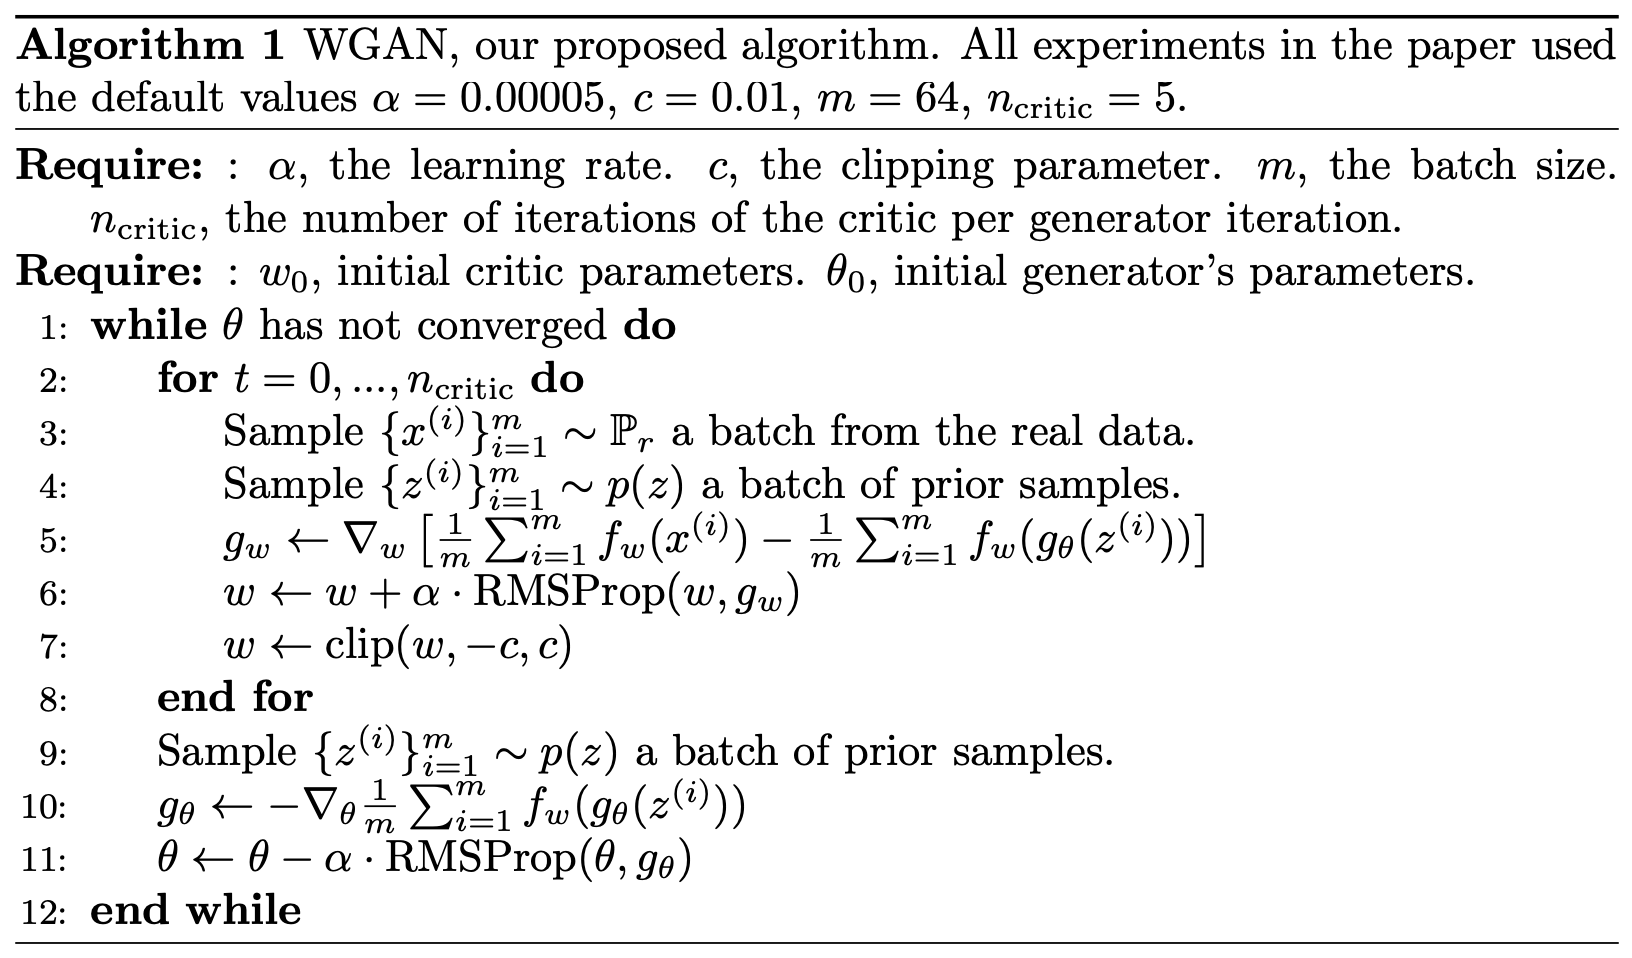
\includegraphics[width=1.0\linewidth]{figs/wgan_pseudocode}
	\end{figure}
	\vfill
	\hrule\medskip 
	{\scriptsize \href{https://arxiv.org/abs/1701.07875}{https://arxiv.org/abs/1701.07875}}
\end{frame}
%=======
\begin{frame}{Wasserstein GAN}
	\begin{figure}
		\centering
		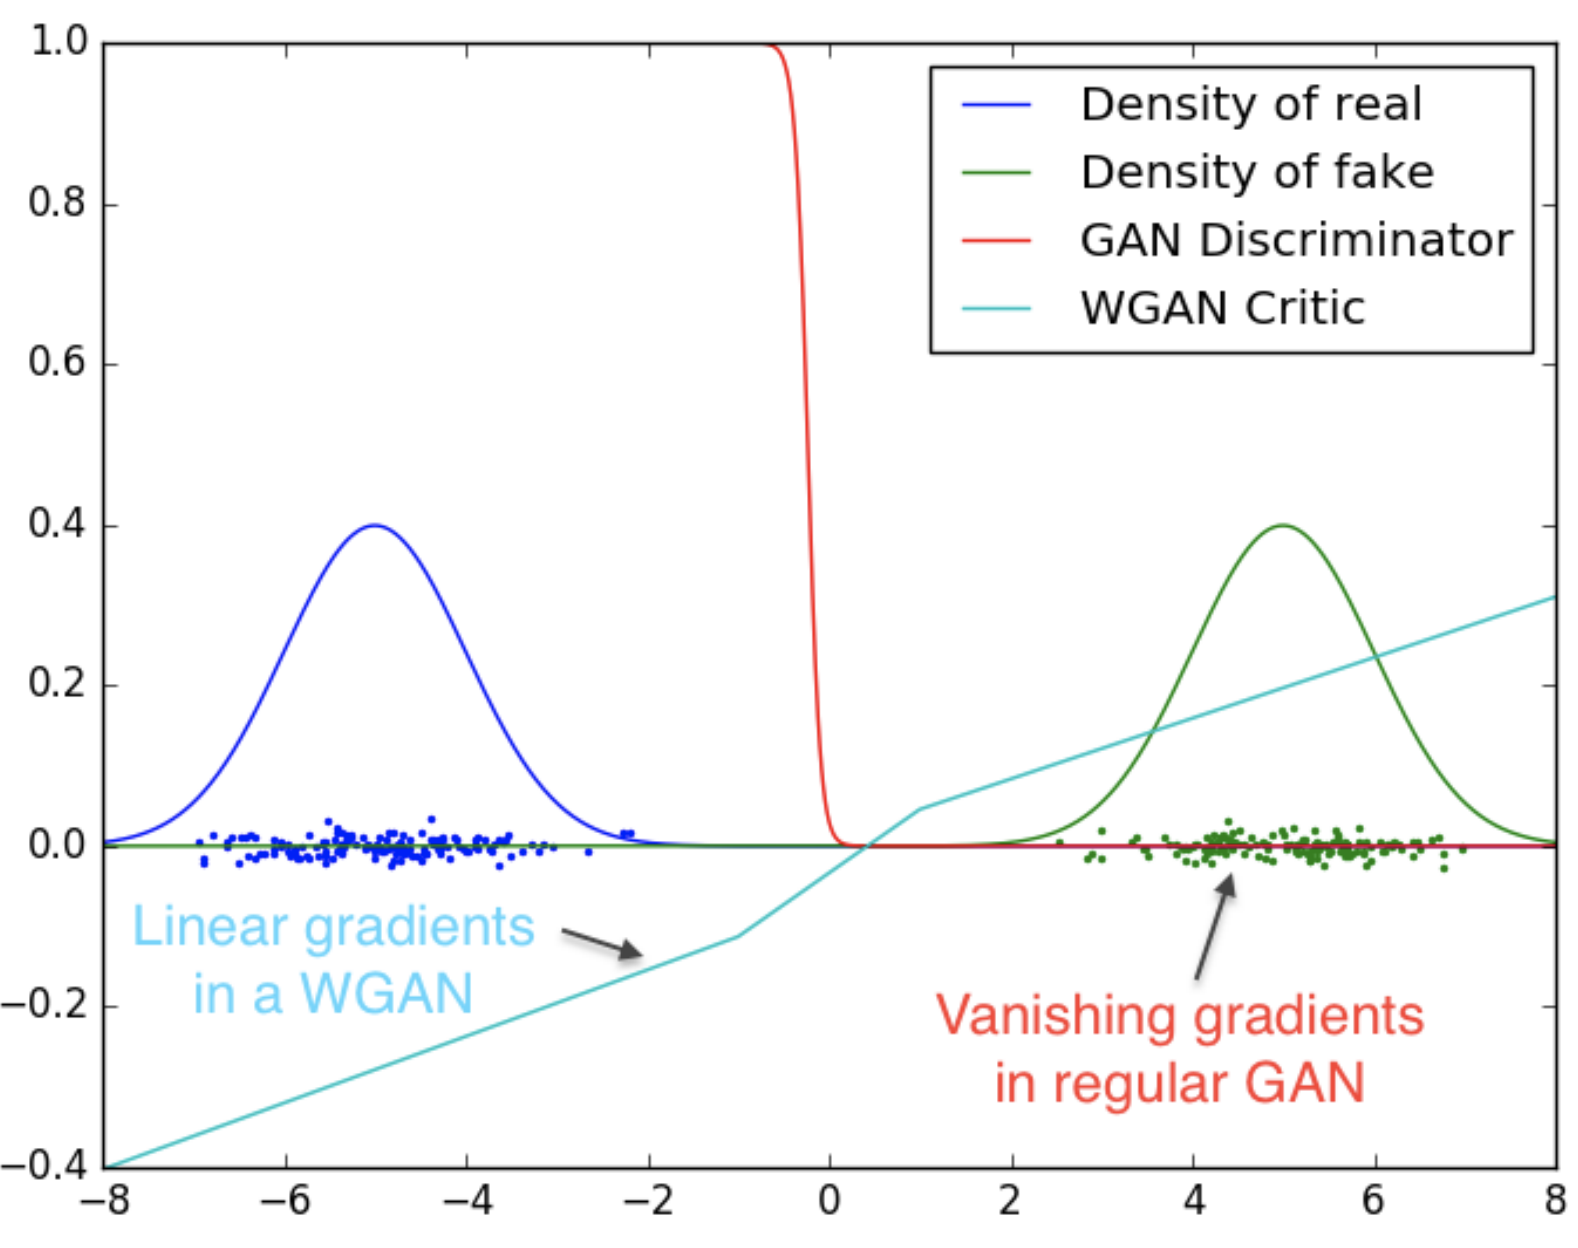
\includegraphics[width=0.8\linewidth]{figs/wgan_toy}
	\end{figure}
	\vfill
	\hrule\medskip 
	{\scriptsize \href{https://arxiv.org/abs/1701.07875}{https://arxiv.org/abs/1701.07875}}
\end{frame}
%=======
\begin{frame}{Wasserstein GAN}
	\begin{minipage}[t]{0.49\columnwidth}
		\begin{figure}
			\centering
			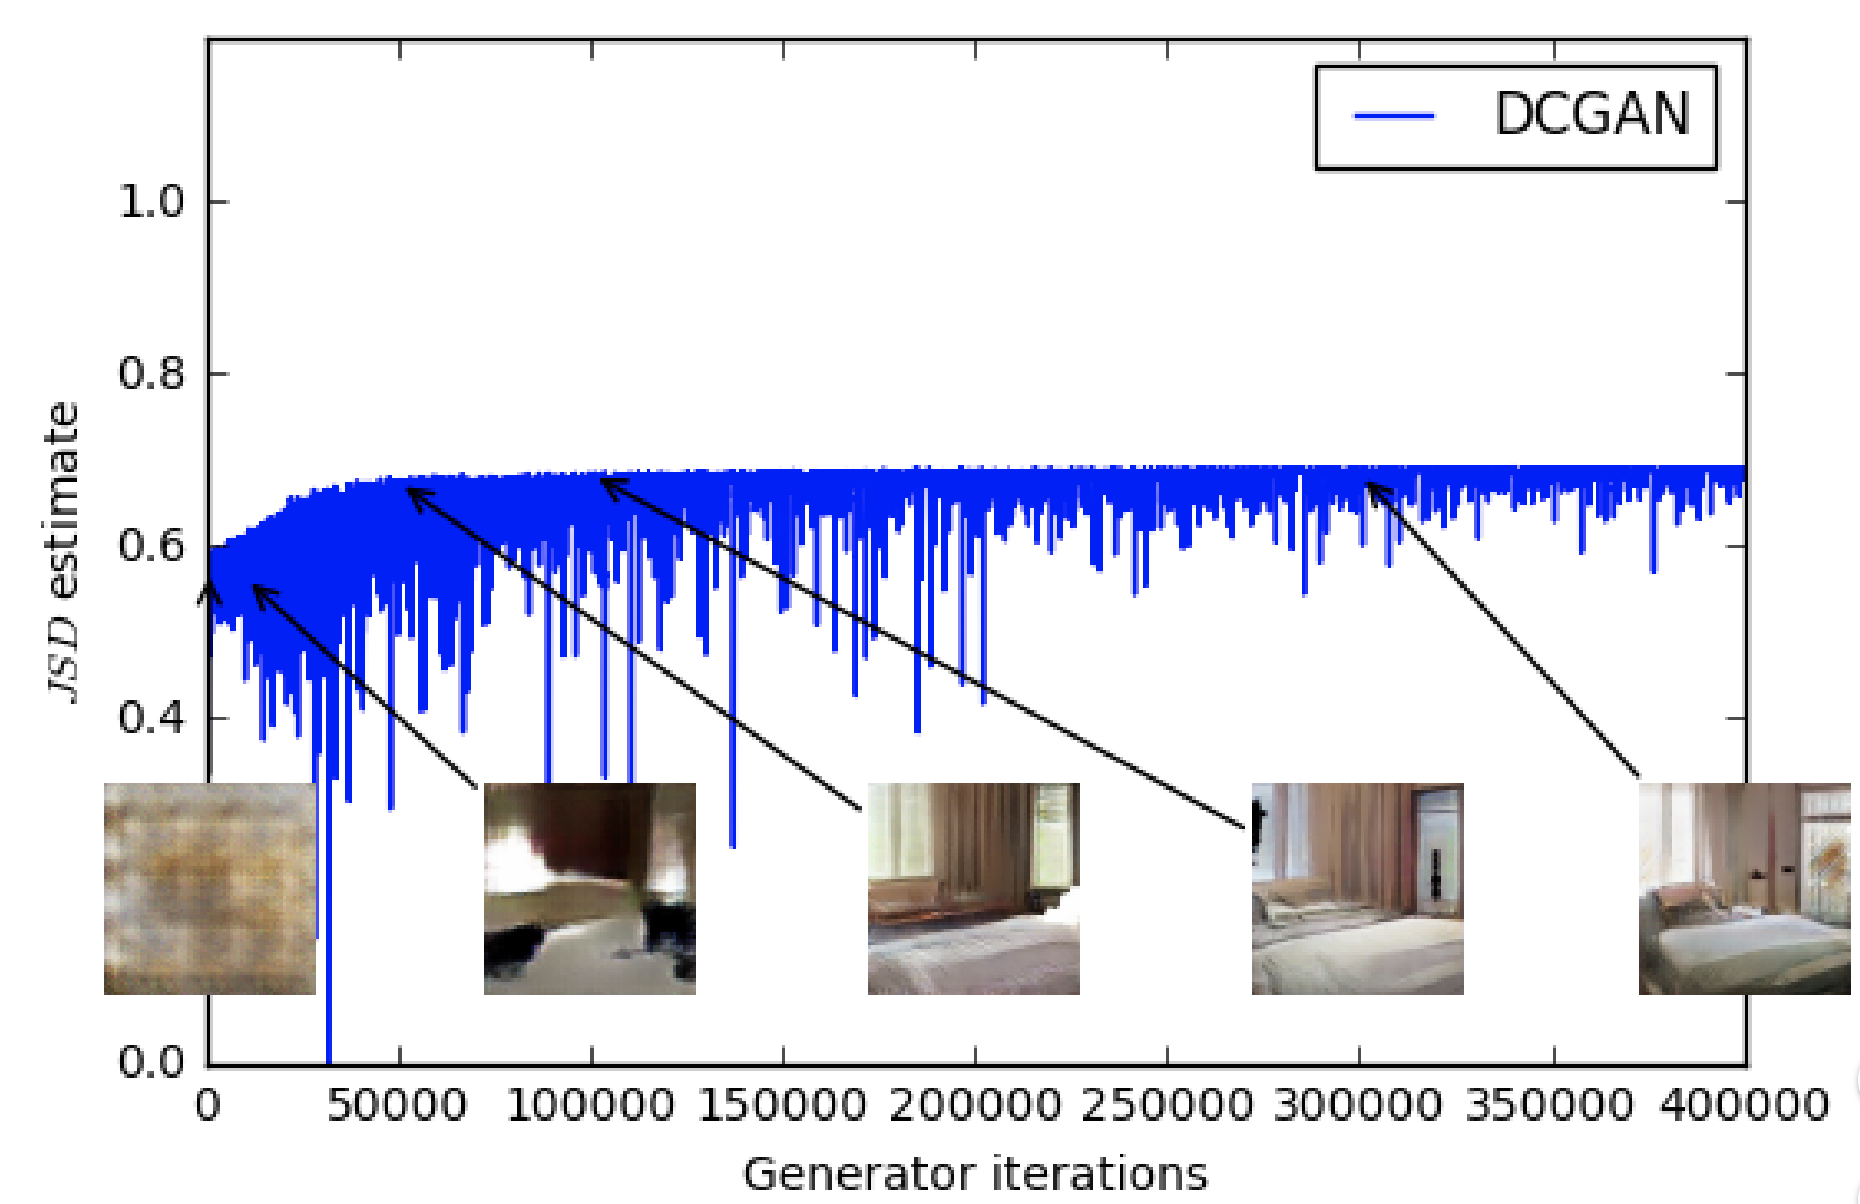
\includegraphics[width=1.0\linewidth]{figs/dcgan_quality}
		\end{figure}
	\end{minipage}%
	\begin{minipage}[t]{0.49\columnwidth}
		\begin{figure}
			\centering
			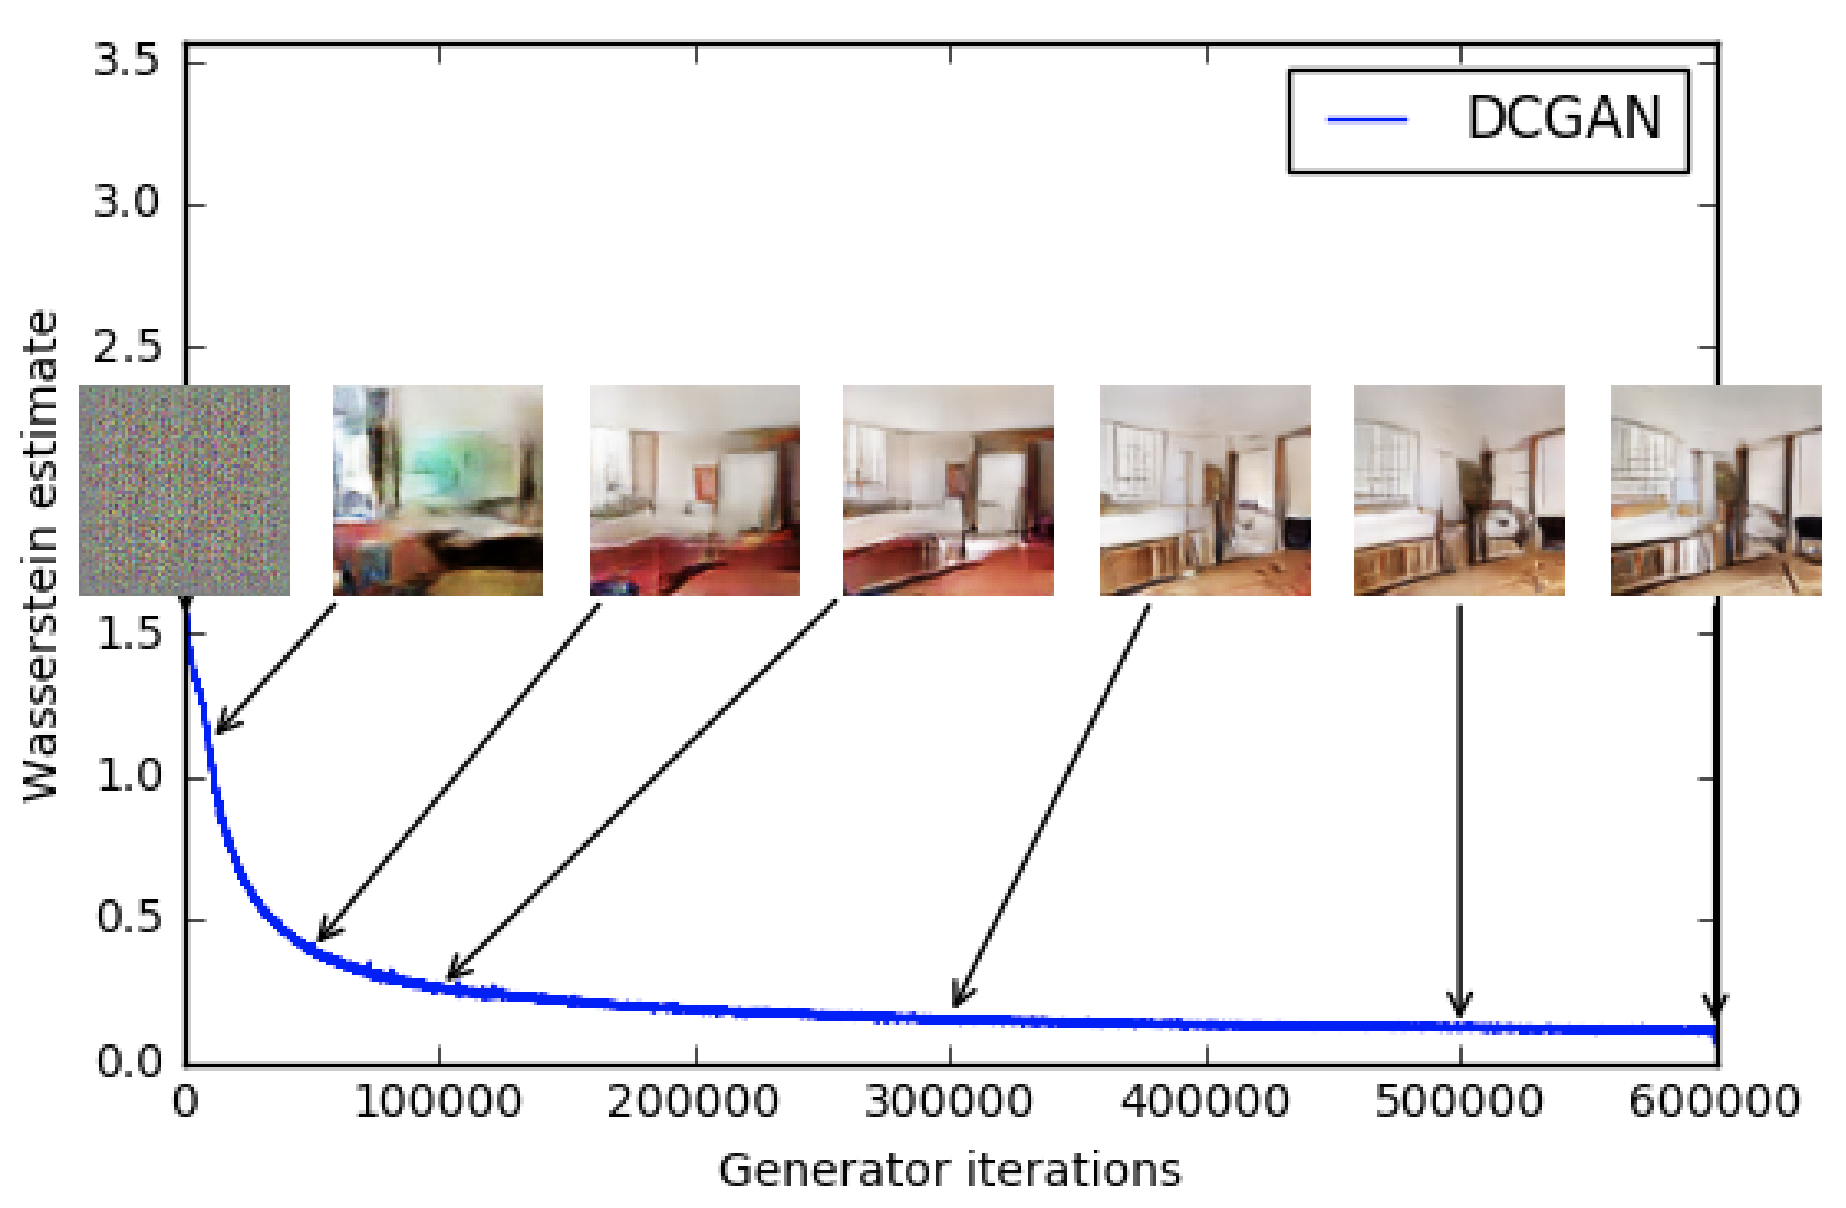
\includegraphics[width=1.0\linewidth]{figs/wgan_quality}
		\end{figure}
	\end{minipage}
	\begin{itemize}
		\item $JSD$ correlates poorly with the sample quality. Stays contast nearly maximum value $\log 2 \approx 0.69$.
		\item $W$ is highly correlated with the sample quality. 
	\end{itemize}
	\vfill
	\hrule\medskip 
	{\scriptsize \href{https://arxiv.org/abs/1701.07875}{https://arxiv.org/abs/1701.07875}}
\end{frame}
%=======
\begin{frame}{Wasserstein GAN}
	\begin{block}{WGAN converged without batch norm and constant number of filters}
		\begin{figure}
			\centering
			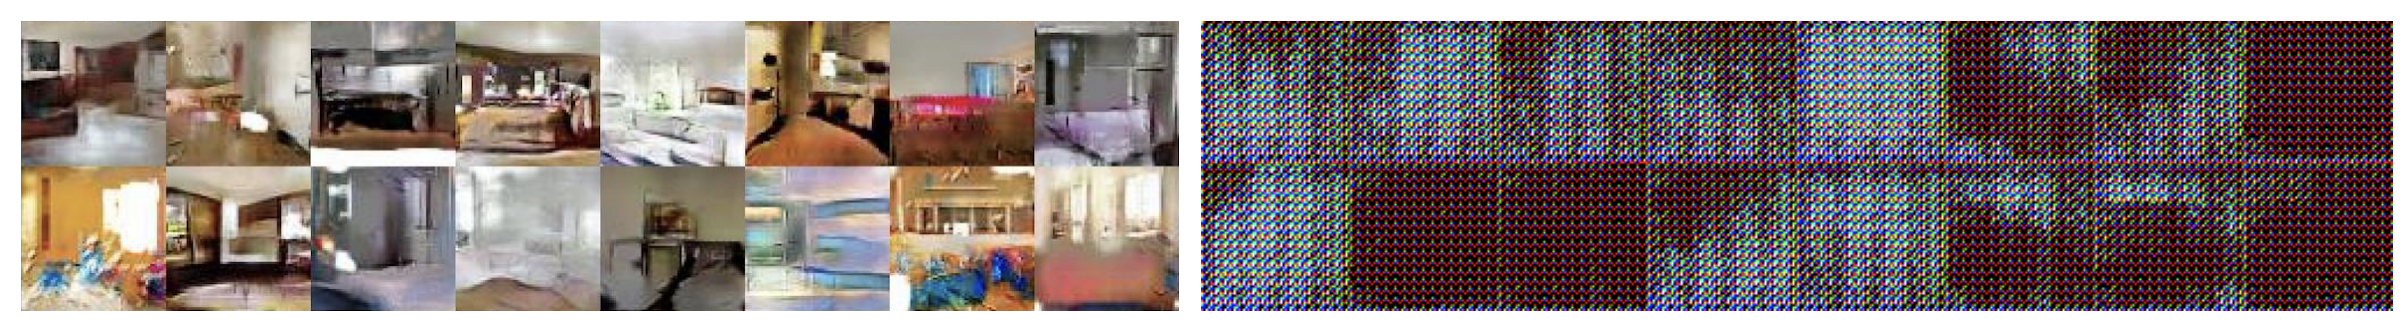
\includegraphics[width=1.0\linewidth]{figs/wgan_convergence}
		\end{figure}
	\end{block}
	\begin{block}{"In no experiment did we see evidence of mode collapse for the WGAN algorithm."}
		\begin{figure}
			\centering
			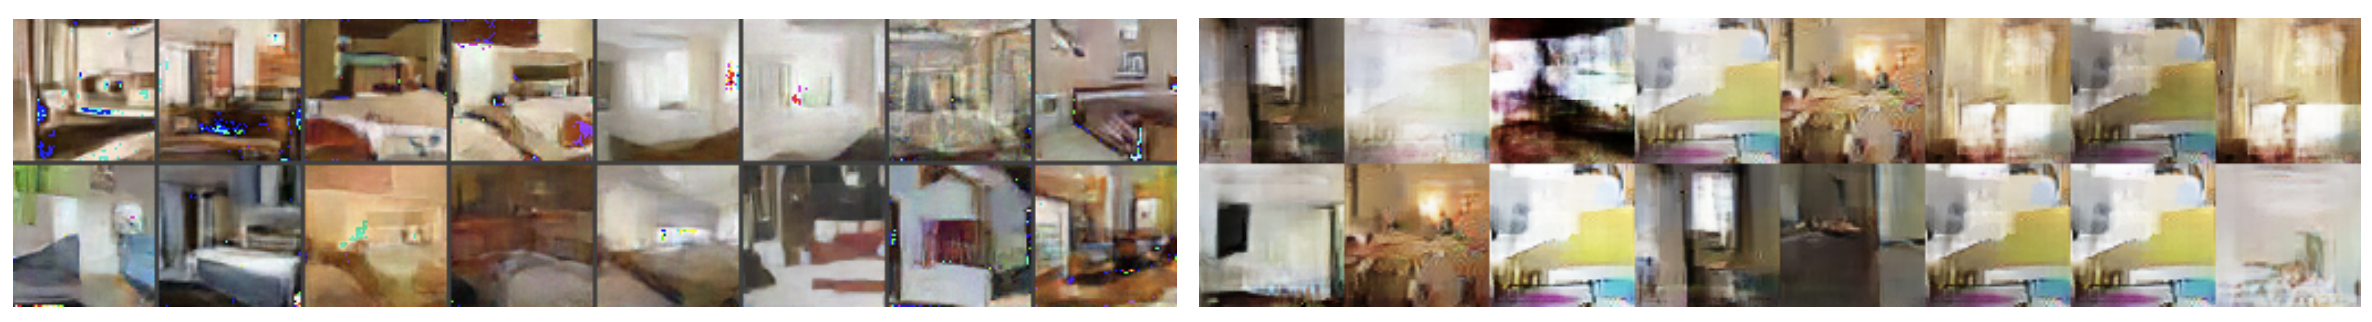
\includegraphics[width=1.0\linewidth]{figs/wgan_mode_collapse}
		\end{figure}
	\end{block}
	\vfill
	\hrule\medskip 
	{\scriptsize \href{https://arxiv.org/abs/1701.07875}{https://arxiv.org/abs/1701.07875}}
\end{frame}
%=======
\begin{frame}{Wasserstein GAN with Gradient Penalty}
	
	\begin{minipage}[t]{0.45\columnwidth}
		\vspace{0.2cm}
		The generator distribution is fixed and equals to the real distribution + Gaussian noise. \\
		Problems with weight clipping:
		\begin{itemize}
			\item The critic ignores higher moments of the data distribution.
			\item The gradient either grow or decay exponentially.
		\end{itemize}
	Gradient penalty makes the gradients  more stable.
	\end{minipage}%
	\begin{minipage}[t]{0.52\columnwidth}
		\begin{figure}
			\centering
			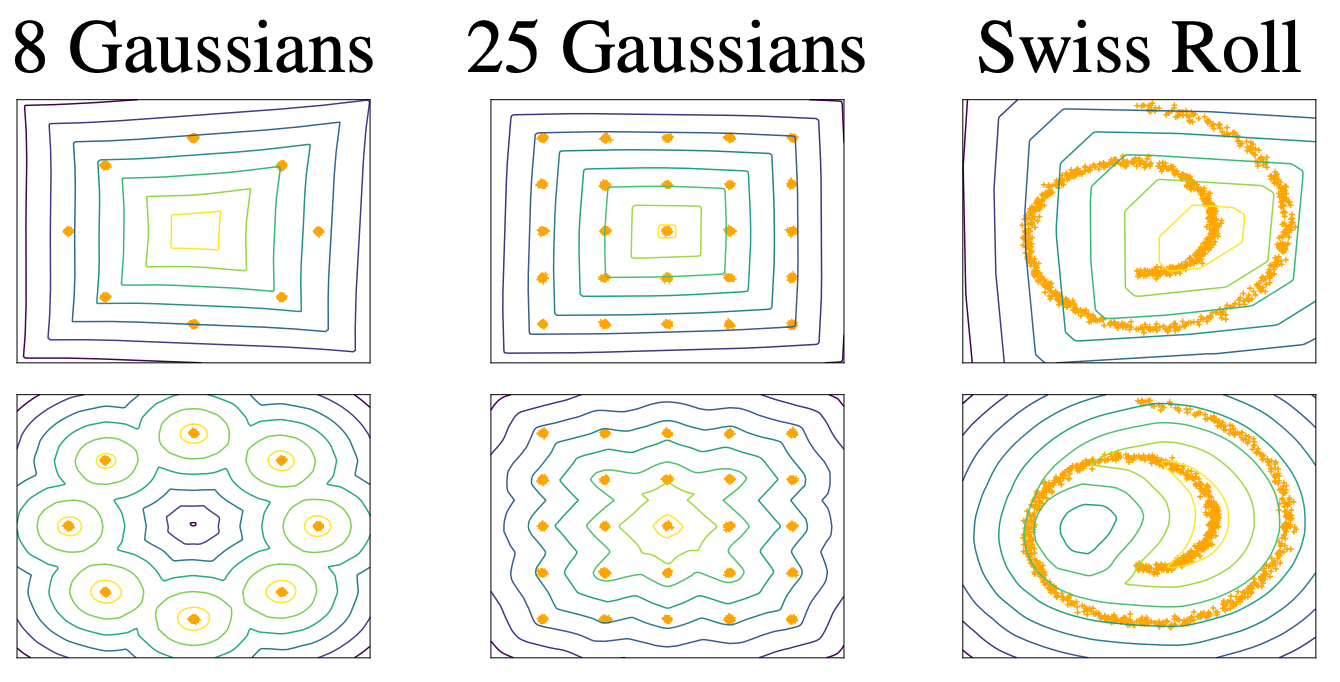
\includegraphics[width=0.95\linewidth]{figs/wgan_gp_toy}
		\end{figure}
		\begin{figure}
			\centering
			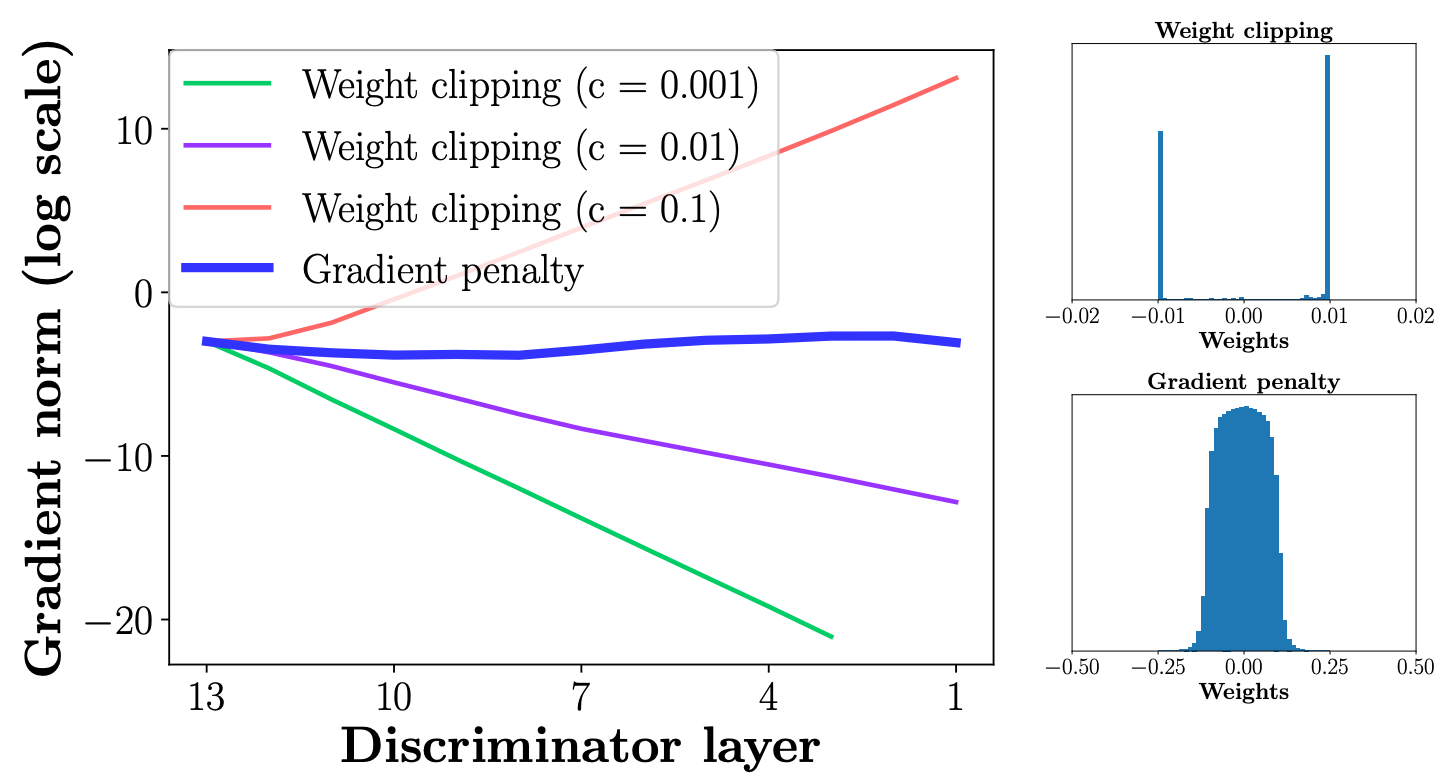
\includegraphics[width=0.95\linewidth]{figs/wgan_gp_weights}
		\end{figure}
	\end{minipage}
	
	\vfill
	\hrule\medskip 
	{\scriptsize \href{https://arxiv.org/abs/1704.00028}{https://arxiv.org/abs/1704.00028}}
	
\end{frame}
%=======
\begin{frame}{Wasserstein GAN with Gradient Penalty}
	\begin{block}{Theorem}
		Let $\pi(\bx)$ and $p(\bx)$ be two distribution in $\cX$, a compact metric space. Then, there is 1-Lipschitz function $f^*$ which is the optimal solution of 
		\[
			\max_{\| f \|_L \leq 1} \left[ \bbE_{\bx \sim \pi} f(\bx)  - \bbE_{\bx \sim p} f(\bx)\right].
		\]
		Let $\gamma$ be the optimal transportation plan between $\pi(\bx)$ and $p(\bx)$. Then, if $f^*$ is differentiable $\gamma(x = y) = 0$ and $\bx_t = t \bx + (1 - t) \by$ with $t \in [0, 1]$ it holds that
		\[
			\bbP_{(\bx, \by) \sim \gamma} \left[ \nabla f^*(\bx_t) = \frac{\by - \bx_t}{\| \by - \bx_t \|} = 1 \right].
		\]
	\end{block}
	\begin{block}{Corollary}
		$f^*$ has gradient norm 1 almost everywhere under $\pi(\bx)$ and $p(\bx)$.
	\end{block}
	\vfill
	\hrule\medskip 
	{\scriptsize \href{https://arxiv.org/abs/1704.00028}{https://arxiv.org/abs/1704.00028}}
\end{frame}
%=======
\begin{frame}{Wasserstein GAN with Gradient Penalty}
	A differentiable function is 1-Lipschtiz if and only if it has gradients with norm at most 1 everywhere.
	\begin{block}{Gradient penalty}
		\[
			W(\pi, p) = \underbrace{\bbE_{\bx \sim \pi} f(\bx)  - \bbE_{\bx \sim p} f(\bx)}_{\text{original critic loss}} + \lambda \underbrace{\bbE_{\hat{\bx}} \left[ \left( \| \nabla_{\hat{\bx}} f(\hat{\bx}) \|_2 - 1 \right) ^ 2\right]}_{\text{gradient penalty}},
		\]
	\end{block}
	\begin{itemize}
		\item Samples $\hat{\bx}$ are uniformly sampled along straight lines between pairs of points from the data distribution $\pi(\bx)$ and the generator distribuiton $p(\bx | \btheta)$.
		\item Enforcing the unit gradient norm constraint everywhere is intractable, it turns out sifficient to enforce it only along these straight lines.
	\end{itemize}
	\vfill
	\hrule\medskip 
	{\scriptsize \href{https://arxiv.org/abs/1704.00028}{https://arxiv.org/abs/1704.00028}}
\end{frame}
%=======
\begin{frame}{Wasserstein GAN with Gradient Penalty}
	
	\begin{figure}
		\centering
		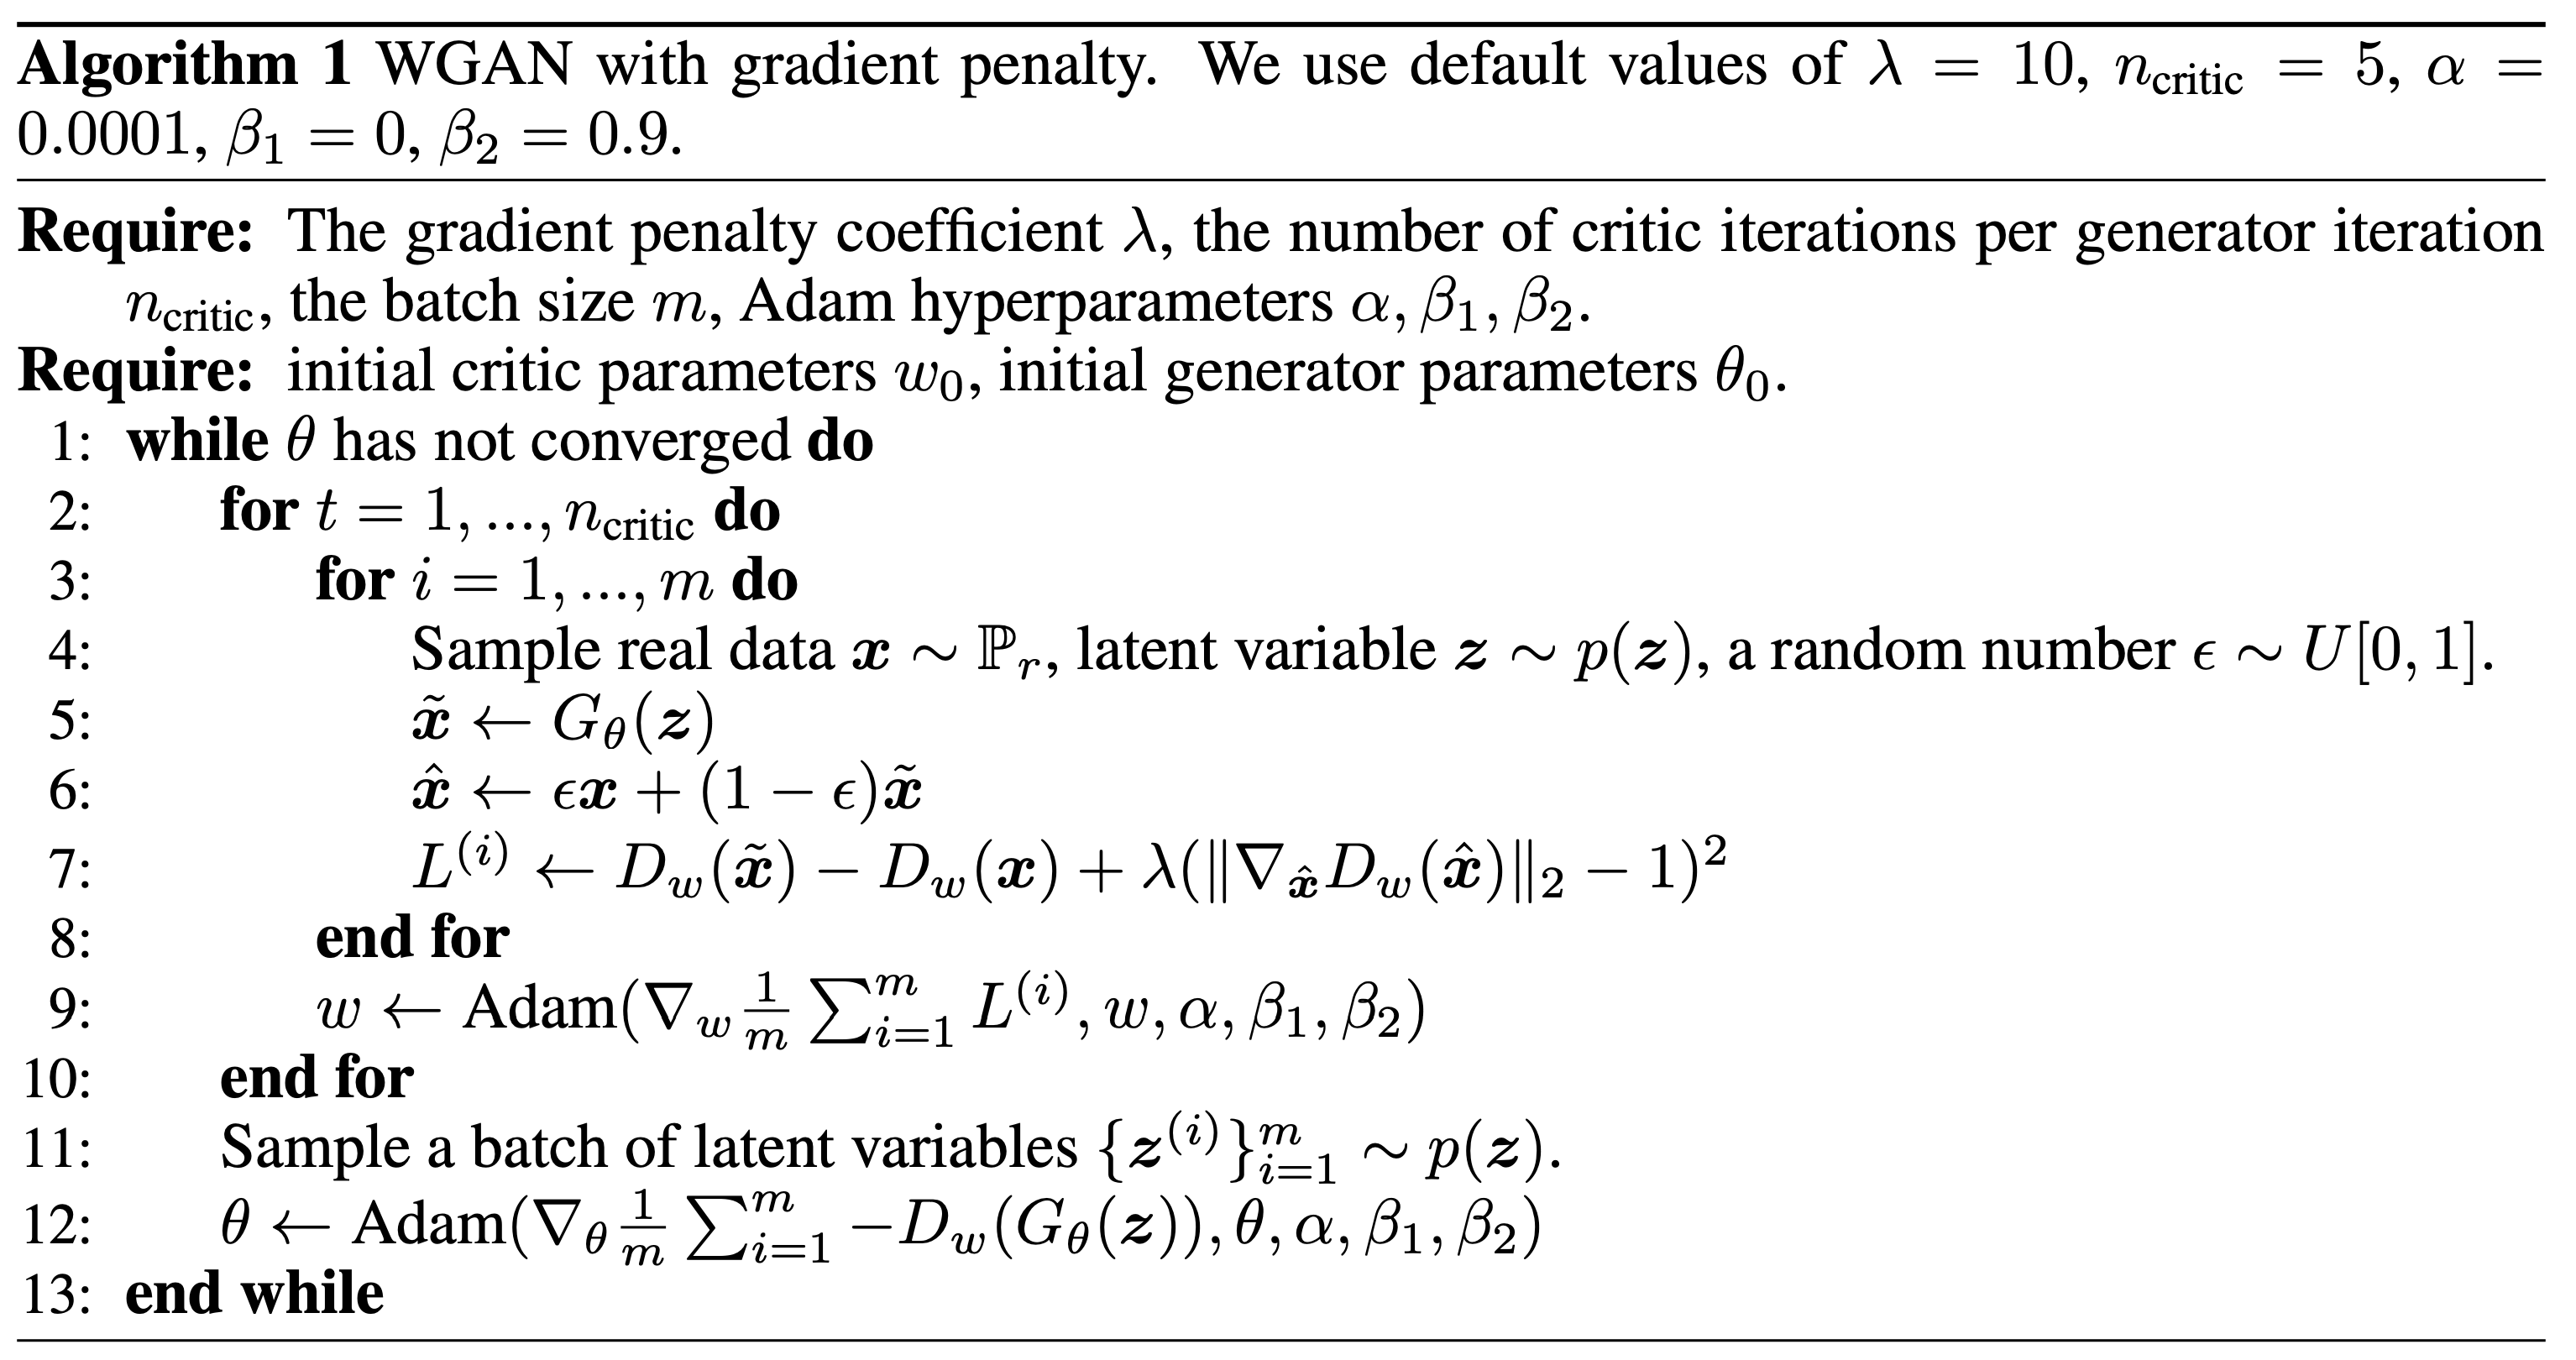
\includegraphics[width=1.0\linewidth]{figs/wgan_gp_pseudocode}
	\end{figure}
	
	\vfill
	\hrule\medskip 
	{\scriptsize \href{https://arxiv.org/abs/1704.00028}{https://arxiv.org/abs/1704.00028}}
	
\end{frame}
%=======
\begin{frame}{Wasserstein GAN with Gradient Penalty}
	\begin{figure}
		\centering
		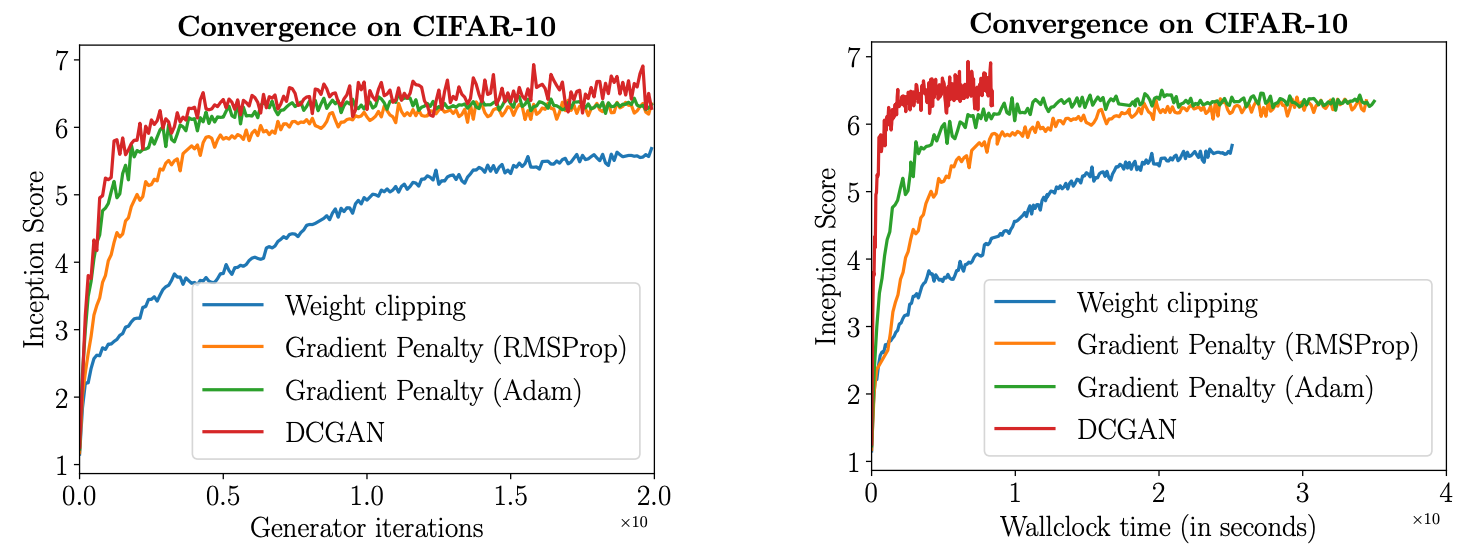
\includegraphics[width=0.9\linewidth]{figs/wgan_gp_convergence}
	\end{figure}
	\begin{figure}
		\centering
		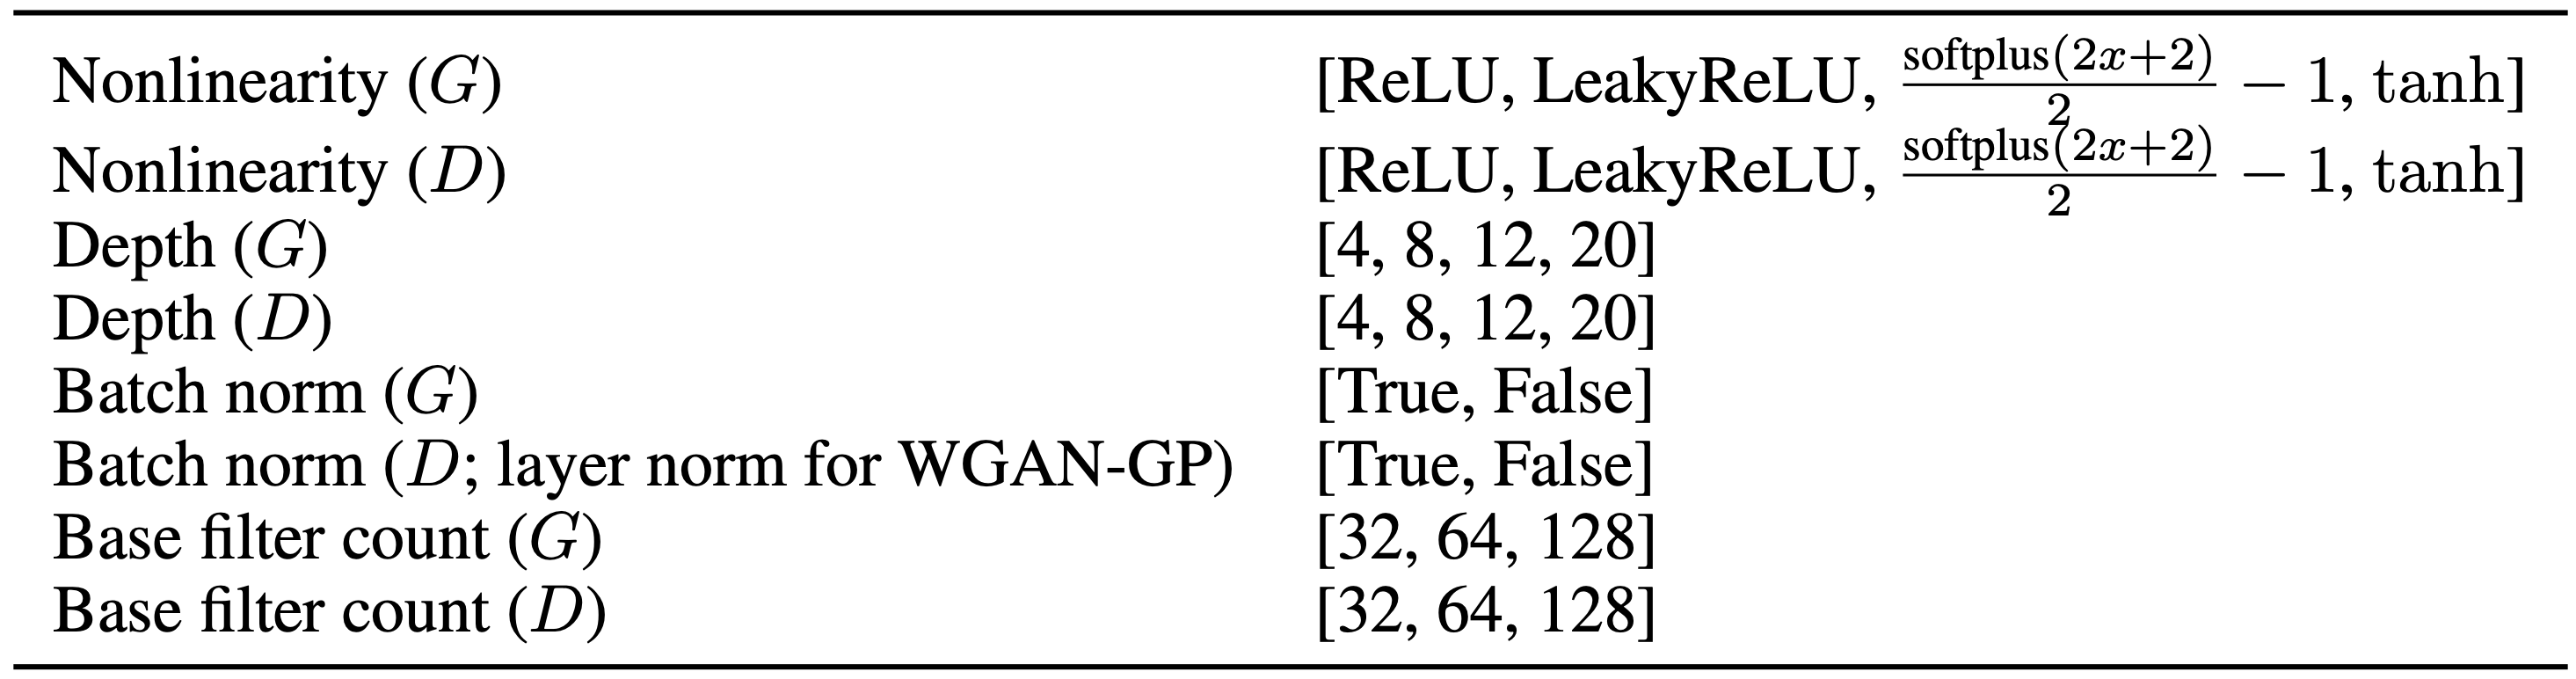
\includegraphics[width=0.65\linewidth]{figs/wgan_gp_model_space}
	\end{figure}
	\begin{figure}
		\centering
		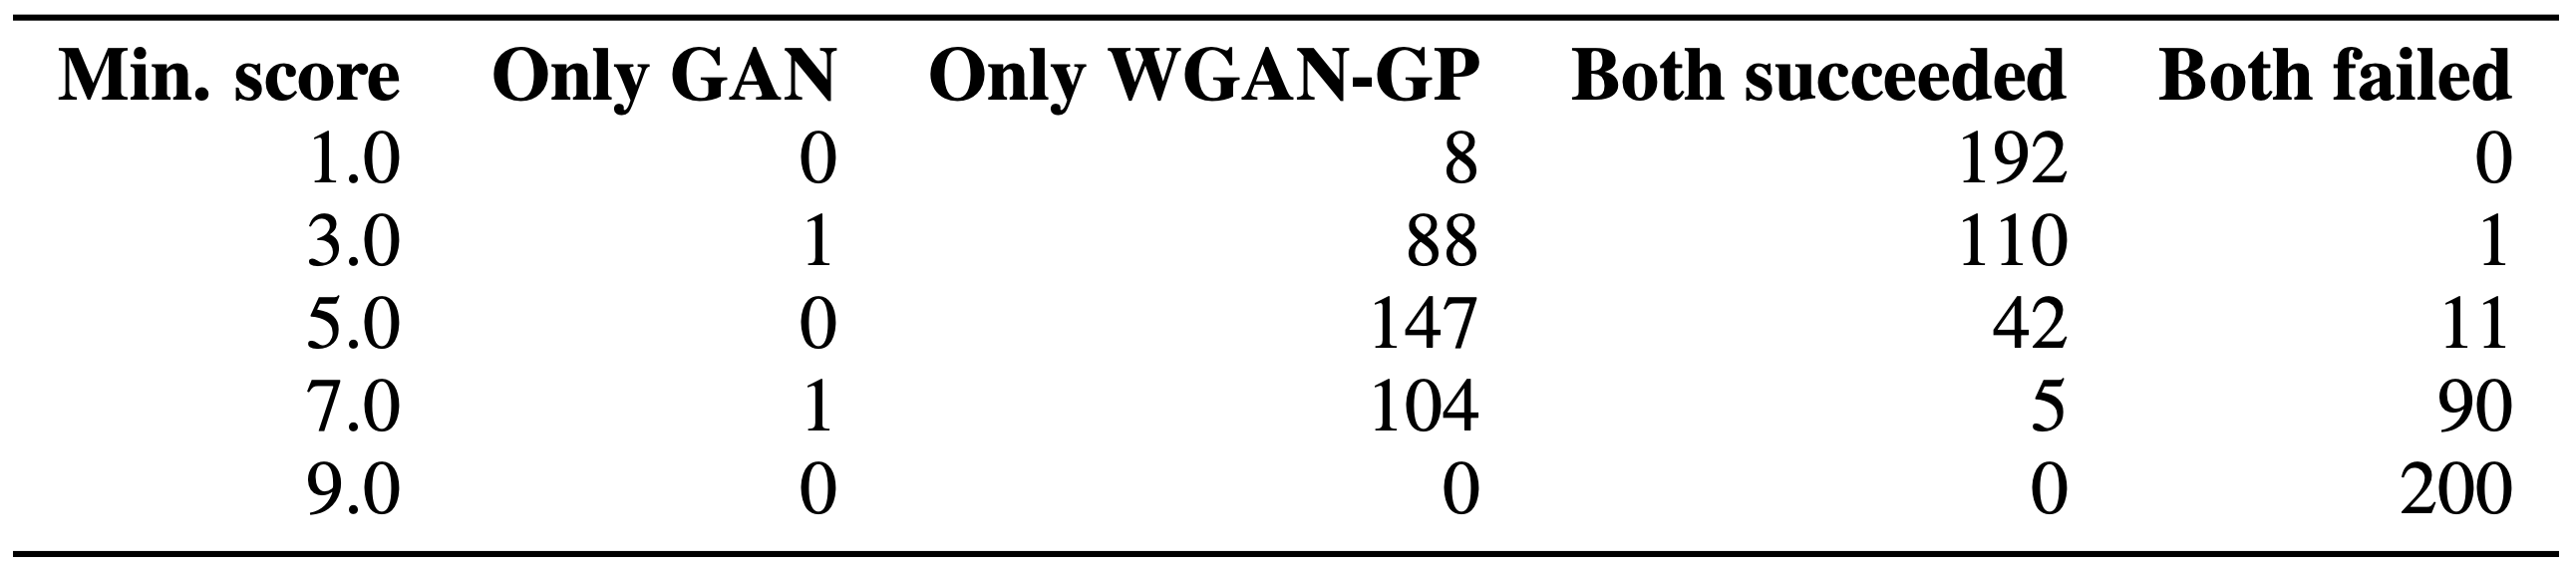
\includegraphics[width=0.65\linewidth]{figs/wgan_gp_wgan}
	\end{figure}
	\vfill
	\hrule\medskip 
	{\scriptsize \href{https://arxiv.org/abs/1704.00028}{https://arxiv.org/abs/1704.00028}}
	
\end{frame}
%=======
\begin{frame}{Wasserstein GAN with Gradient Penalty}
	\begin{figure}
		\centering
		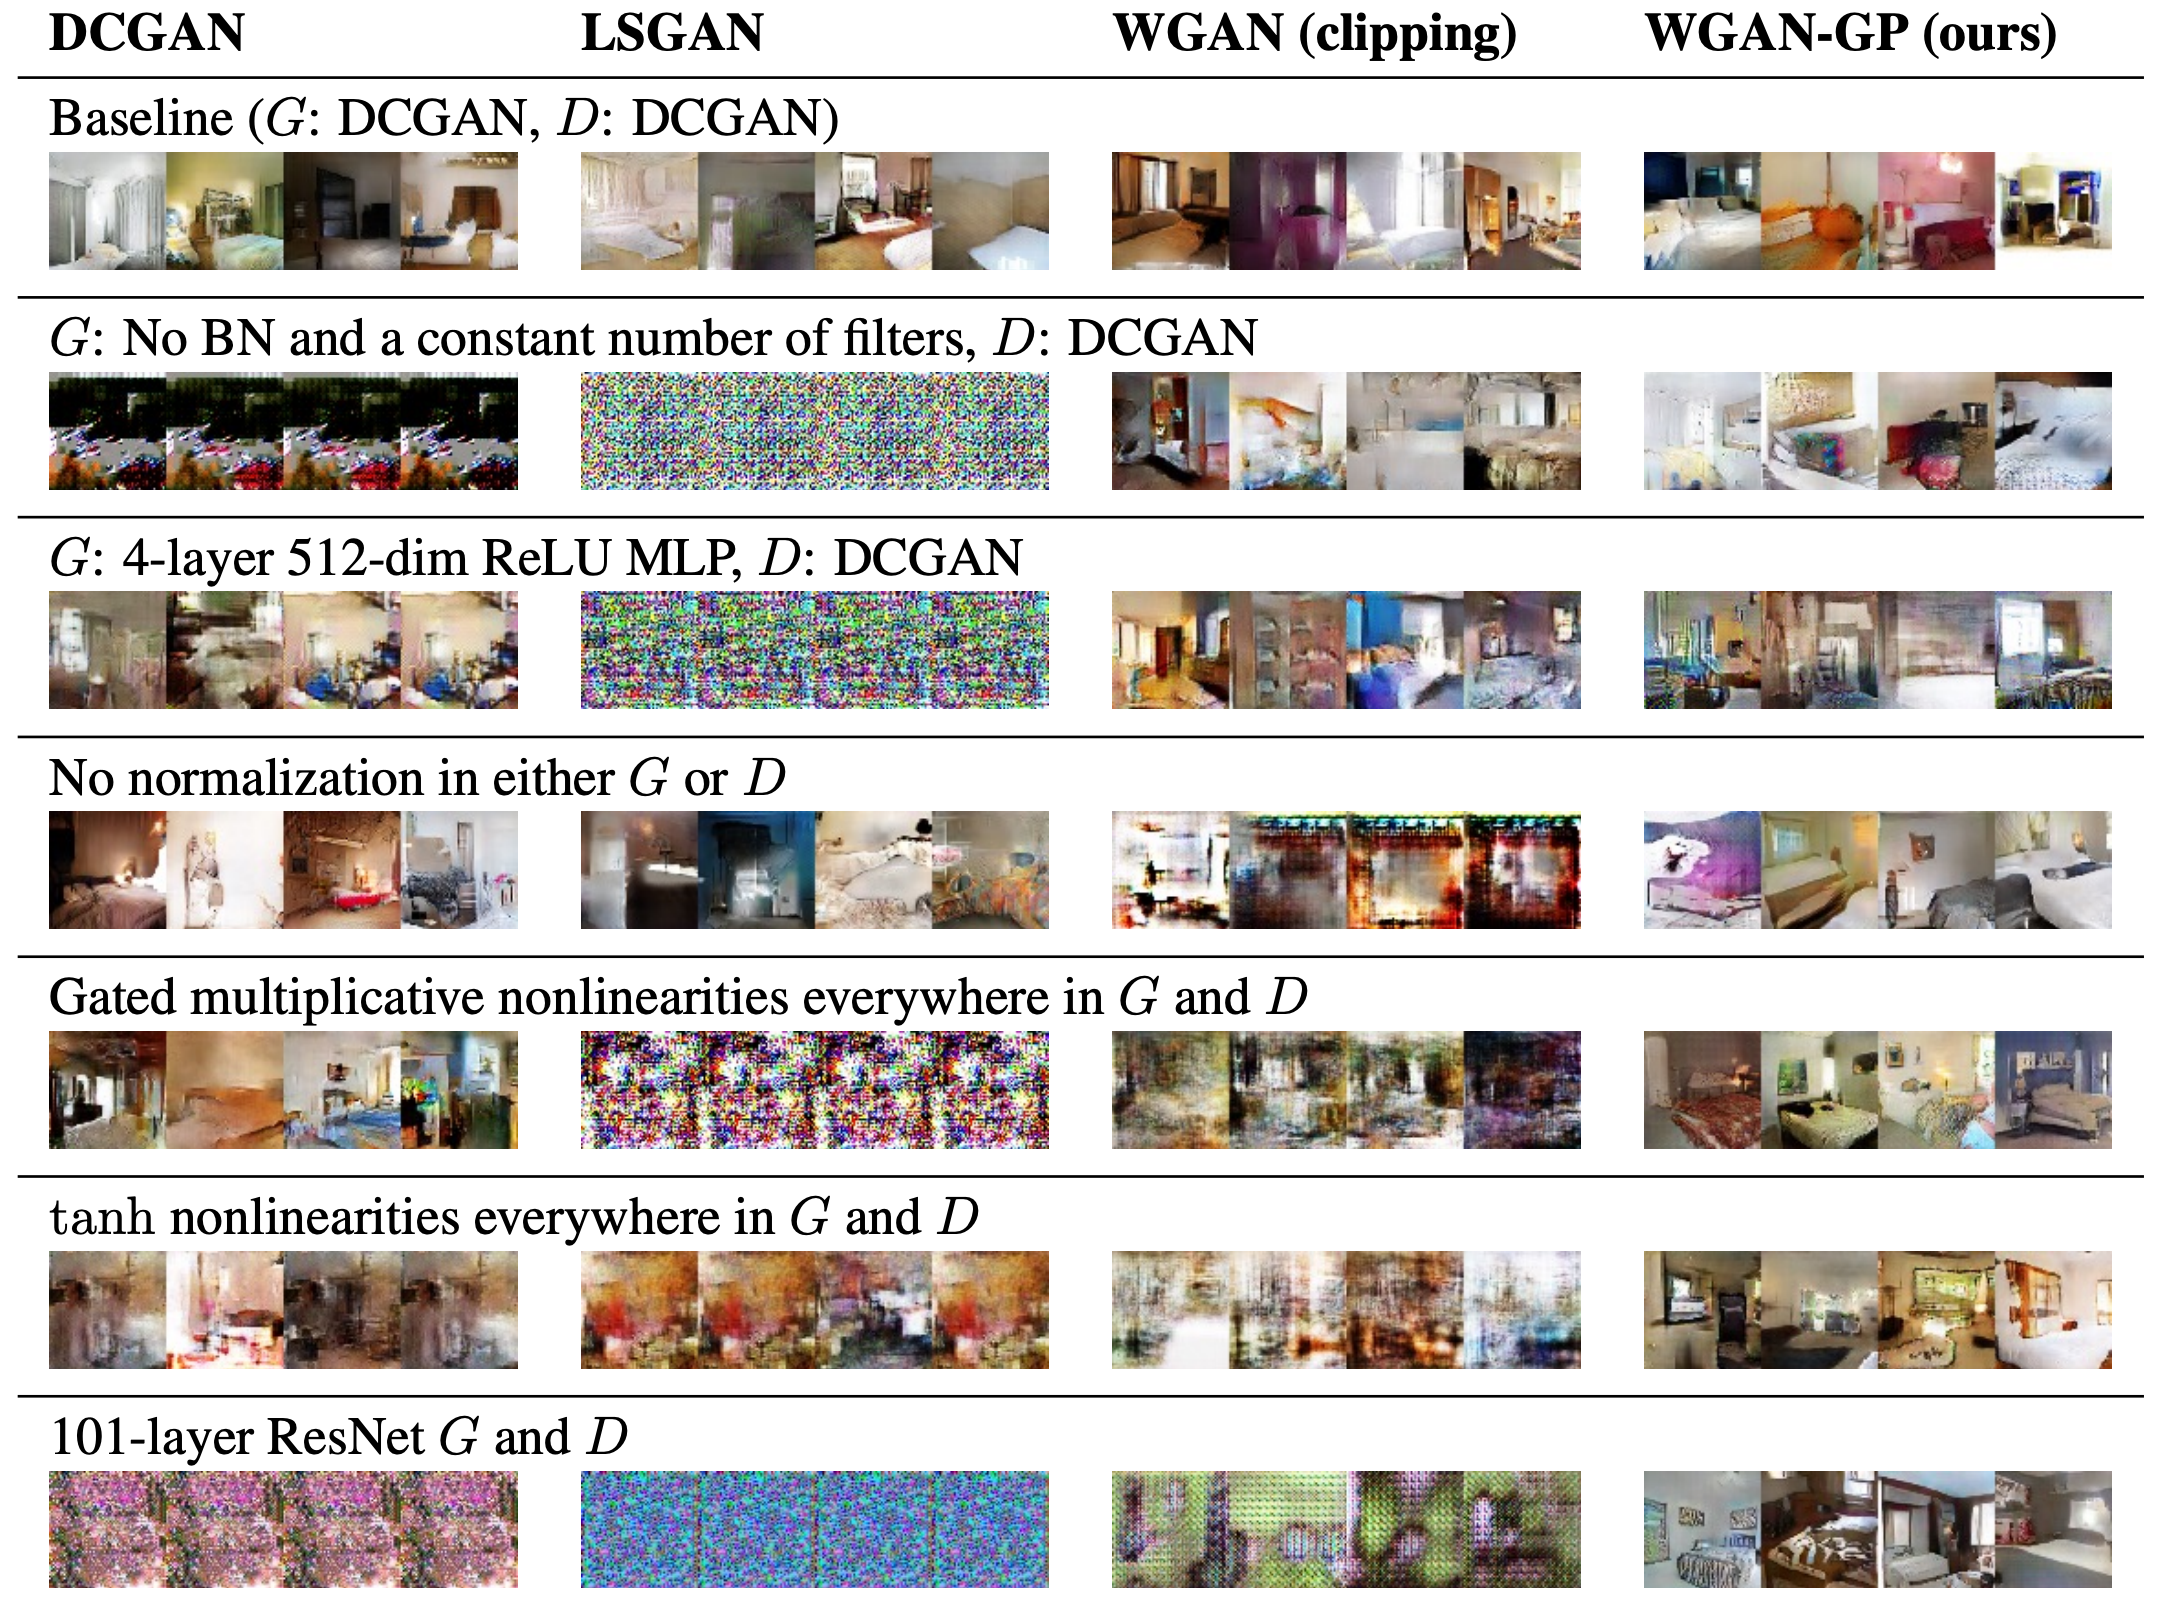
\includegraphics[width=0.95\linewidth]{figs/wgan_gp_results}
	\end{figure}
	\vfill
	\hrule\medskip 
	{\scriptsize \href{https://arxiv.org/abs/1704.00028}{https://arxiv.org/abs/1704.00028}}
	
\end{frame}
%=======
\begin{frame}{Spectral Normalization GAN}
	How else could we enforce Lipschitzness?
	\begin{block}{Fact 1}
		\vspace{-0.3cm}
		\[
			\| \mathbf{g} \|_L = \sup_\bx \sigma( \nabla \mathbf{g}(\bx))
		\]
	\end{block}
	Here $\sigma(\bA)$~-- spectral norm of matrix $\bA$.
	\[
		\sigma(\bA) = \max_{\bh \neq 0} \frac{\|\bA \bh\|_2}{\|\bh\|_2} = \max_{\|\bh\|_2 \leq 1} \| \bA \bh \|_2 = \lambda_{\text{max}}(A),
	\]
	where $\lambda_{\text{max}}(A)$ is the largest singular value of $\bA$.
	\begin{block}{Fact 2}
		\vspace{-0.3cm}
		\[
			\| \mathbf{g}_1 \circ \mathbf{g}_2 \|_L \leq \| \mathbf{g}_1 \|_L \cdot \| \mathbf{g}_2\|_L
		\]
	\end{block}
	\vfill
	\hrule\medskip 
	{\scriptsize \href{https://arxiv.org/abs/1802.05957}{https://arxiv.org/abs/1802.05957}}
	
\end{frame}
%=======
\begin{frame}{Spectral Normalization GAN}
	Let consider the critic $f(\bx, \bphi)$ of the following form:
	\[
		f(\bx, \bphi) = \bW_{K+1} a_K (\bW_K a_{K-1}(\dots a_1(\bW_1 \bx) \dots)).
	\]
	This feedforward network is a superposition of simple functions.
	\begin{itemize}
		\item $a_k$ is a pointwise nonlinearities. We assume that $\| a_k \|_L = 1$ (it holds for ReLU).
		\item $\mathbf{g}(\bh) = \bW \bh$ is a linear transformation.
		\[
			\| \mathbf{g} \|_L = \sup_\bx \sigma( \nabla \mathbf{g}(\bx)) = \sigma(\bW).
		\]
	\end{itemize}
	\vspace{-0.5cm}
	\begin{block}{Critic spectral norm}
		\vspace{-0.5cm}
		\[
			\| f \|_L \leq \prod_{k=1}^{K+1} \sigma(\bW_k).
		\]
	\end{block}
	If we replace the weights in the critic by $\bW^{SN}_k = \bW_k / \sigma(\bW_k)$, we will get $\| f\|_L \leq 1.$ \\
	
	\vspace{0.1cm}
	\vfill
	\hrule\medskip 
	{\scriptsize \href{https://arxiv.org/abs/1802.05957}{https://arxiv.org/abs/1802.05957}}
\end{frame}
%=======
\begin{frame}{Spectral Normalization GAN}
	 If we apply singular value decomposition to compute the $\sigma(\bW)$ at each round of the algorithm, the algorithm becomes computationally heavy.
	 \begin{block}{Power iteration}
	 	\begin{itemize}
	 		\item $\bu$ -- random vector.
	 		\item repeat
	 		\[
	 			\bv = \frac{\bW^T \bu}{\| \bW^T \bu \|}, \quad \bu = \frac{\bW \bv}{\| \bW \bv \|}
	 		\]
	 		\item approximate the spectral norm
	 		\[
	 			\sigma(\bW) \approx \bu^T \bW \bv
	 		\]
	 	\end{itemize}
	 \end{block}
	\vfill
	\hrule\medskip 
	{\scriptsize \href{https://arxiv.org/abs/1802.05957}{https://arxiv.org/abs/1802.05957}}
\end{frame}
%=======
\begin{frame}{Spectral Normalization GAN}
	\begin{figure}
		\centering
		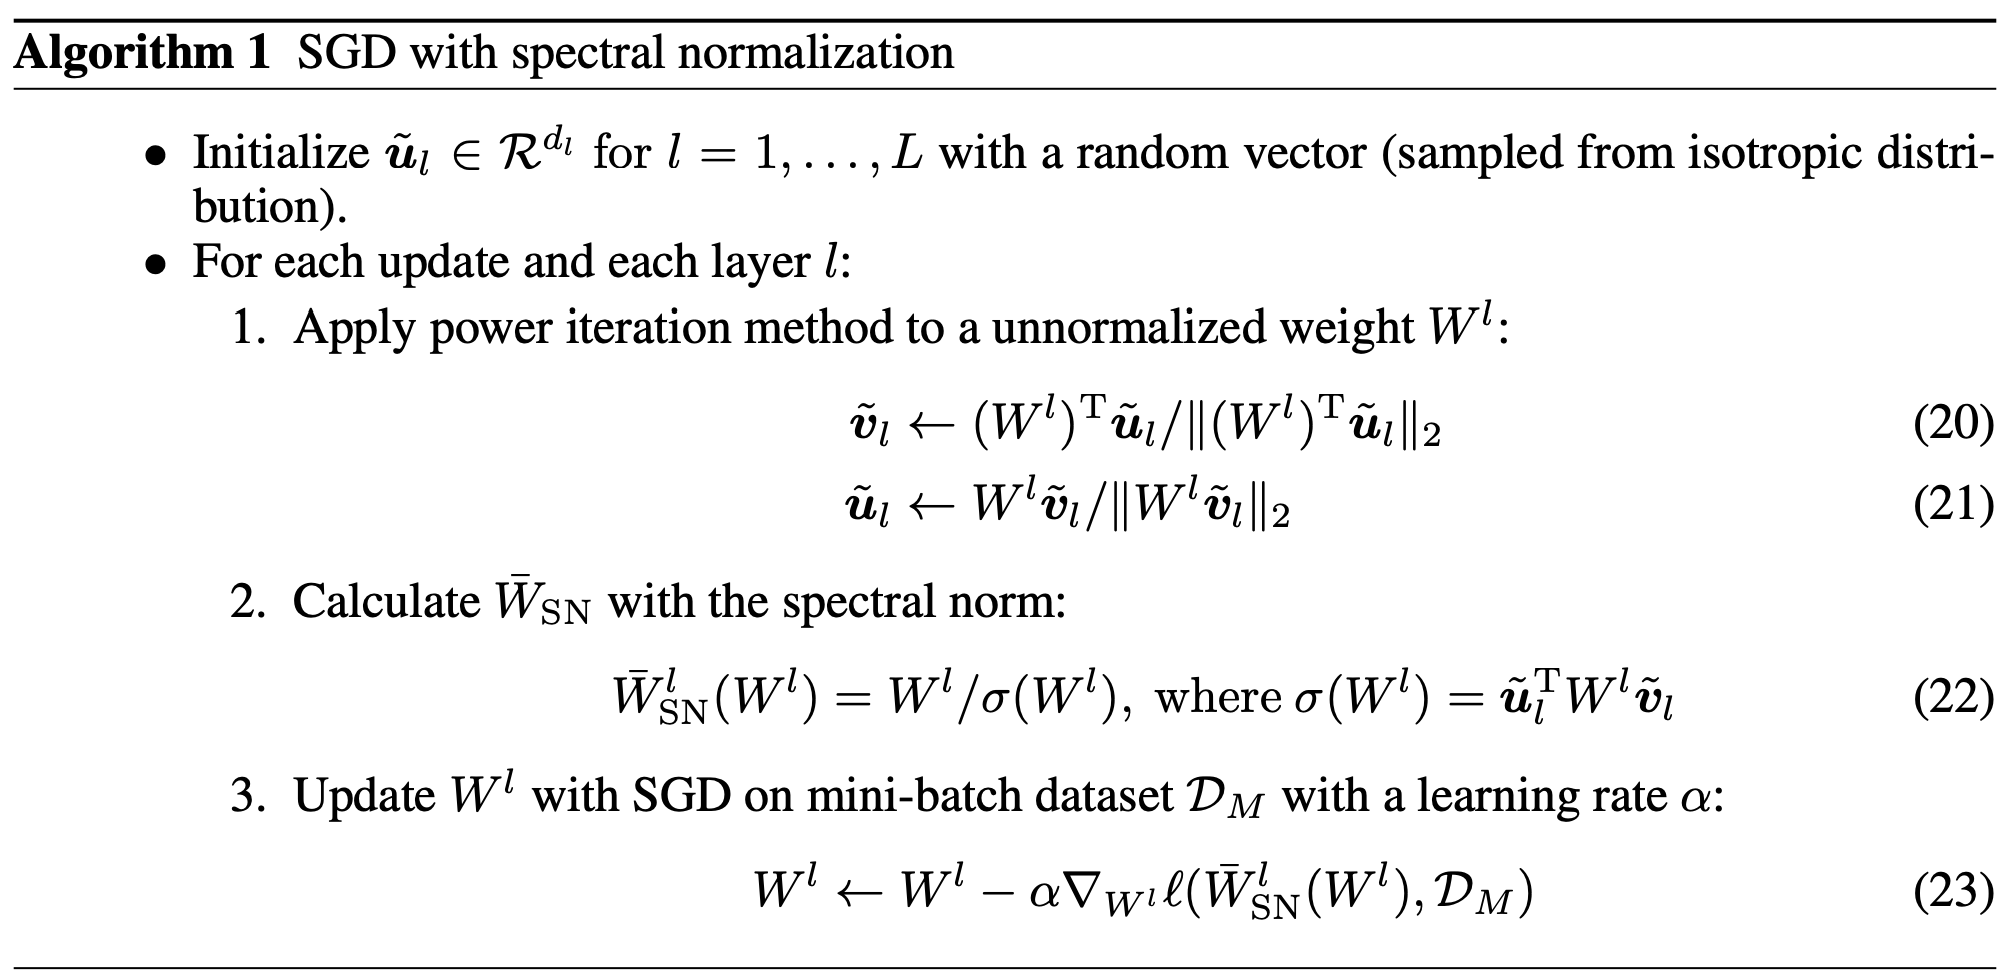
\includegraphics[width=0.85\linewidth]{figs/sngan_pseudocode}
	\end{figure}
	\begin{figure}
		\centering
		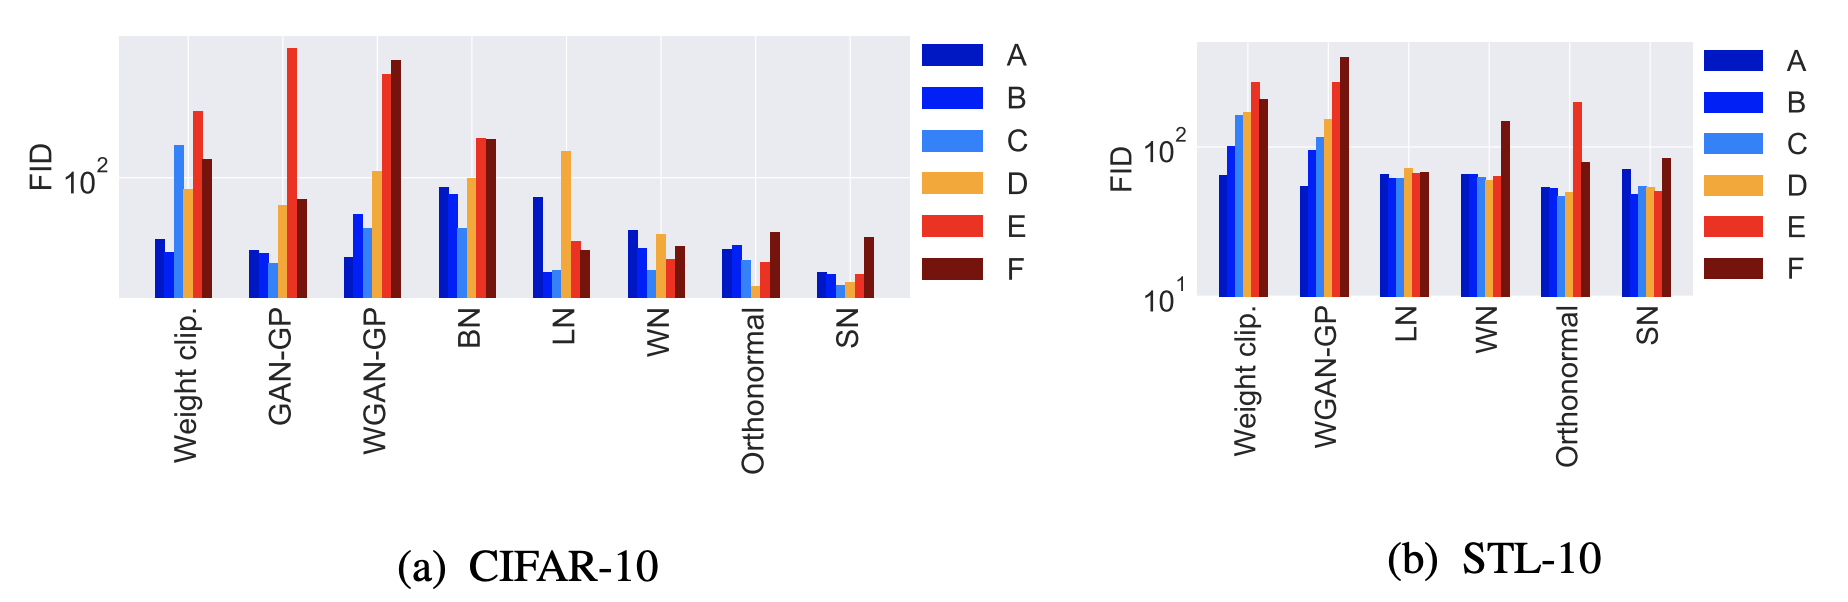
\includegraphics[width=0.85\linewidth]{figs/sngan_fids}
	\end{figure}
	\vfill
	\hrule\medskip 
	{\scriptsize \href{https://arxiv.org/abs/1802.05957}{https://arxiv.org/abs/1802.05957}}
\end{frame}
%=======
\begin{frame}{Divergences}
	\begin{block}{What do we have?}
		\begin{itemize}
			\item Forward KL divergence in maximum likelihood estimation
			\item Reverse KL in variational inference
			\item JS divergence in  vanilla gan
			\item Wasserstein distance in WGAN
		\end{itemize}
	\end{block}
	\begin{block}{Divergence minimization}
		\vspace{-0.3cm}
		\[
			\min_p D(\pi || p)
		\]
		\vspace{-0.5cm}
	\end{block}
	\begin{block}{What is a divergence?}
		Let $\cS$ be the set of all possible probability distributions. Then $D: \cS \times \cS \rightarrow \bbR$ is a divertgence if 
		\begin{itemize}
			\item $D(\pi || p) \geq 0$ for all $\pi, p \in \cS$;
			\item $D(\pi || p) = 0$ if and only if $\pi \equiv p$.
		\end{itemize}
	\end{block}
\end{frame}
%=======
\begin{frame}{f-divergence family}
	
	\begin{block}{f-divergence}
		\vspace{-0.3cm}
		\[
		D_f(\pi || p) = \bbE_p  f\left( \frac{\pi(\bx)}{p(\bx)} \right)  = \int p(\bx) f\left( \frac{\pi(\bx)}{p(\bx)} \right) d \bx.
		\]
		Here $f: \bbR_+ \rightarrow \bbR$ is a convex, lower-semicontinuous function satisfying $f(1) = 0$.
	\end{block}
	\begin{block}{Fenchel conjugate}
		\vspace{-0.5cm}
		\[
		f^*(t) = \sup_{u \in \text{dom}_f} \left( ut - f(u) \right), \quad f^{**} = f, \quad f(u) = \sup_{t \in \text{dom}_{f^*}} \left( ut - f^*(t) \right)
		\]
		\vspace{-0.5cm}
	\end{block}
	\begin{figure}
		\centering
		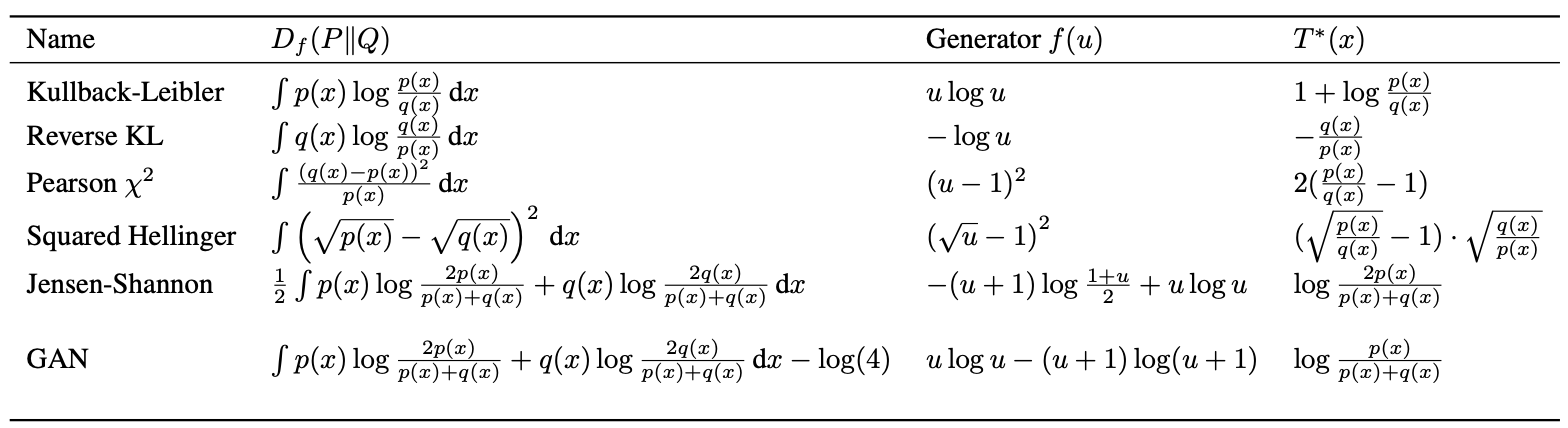
\includegraphics[width=0.85\linewidth]{figs/f_divs}
	\end{figure}
	\vfill
	\hrule\medskip 
	{\scriptsize \href{https://arxiv.org/abs/1606.00709}{https://arxiv.org/abs/1606.00709}}
\end{frame}
%=======
\begin{frame}{f-divergence family}
	\begin{block}{Variational divergence estimation}
		\vspace{-0.3cm}
		\begin{align*}
			D_f(\pi || p) &= \int p(\bx) f\left( \frac{\pi(\bx)}{p(\bx)} \right) d \bx \\
			& = \int p(\bx) \sup_{t \in \text{dom}_{f^*}} \left( \frac{\pi(\bx)}{p(\bx)} t - f^*(t) \right) d \bx \\
			& = \int \sup_{t \in \text{dom}_{f^*}} \left( \pi(\bx)t - p(\bx) f^*(t) \right) d \bx \\
			& \geq \sup_{T \in \cT} \int \left( \pi(\bx)T(\bx) - p(\bx) f^*(T(\bx)) \right) d \bx \\
			& = \sup_{T \in \cT} \left[\bbE_{\pi}T(\bx) -  \bbE_p f^*(T(\bx)) \right]
		\end{align*}
	\end{block}
	Here $\cT: \cX \rightarrow \bbR$ is an arbitrary class of functions.
	
	The lower bound is tight for $T^*(\bx) = f'\left( \frac{\pi(\bx)}{p(\bx)} \right)$.
	\vfill
	\hrule\medskip 
	{\scriptsize \href{https://arxiv.org/abs/1606.00709}{https://arxiv.org/abs/1606.00709}}
\end{frame}
%=======
\begin{frame}{f-divergence family}
	\begin{block}{Variational divergence estimation}
		\[
			D_f(\pi || p) \geq \sup_{T \in \cT} \left[\bbE_{\pi}T(\bx) -  \bbE_p f^*(T(\bx)) \right]
		\]
	\end{block}
	\begin{figure}
		\centering
		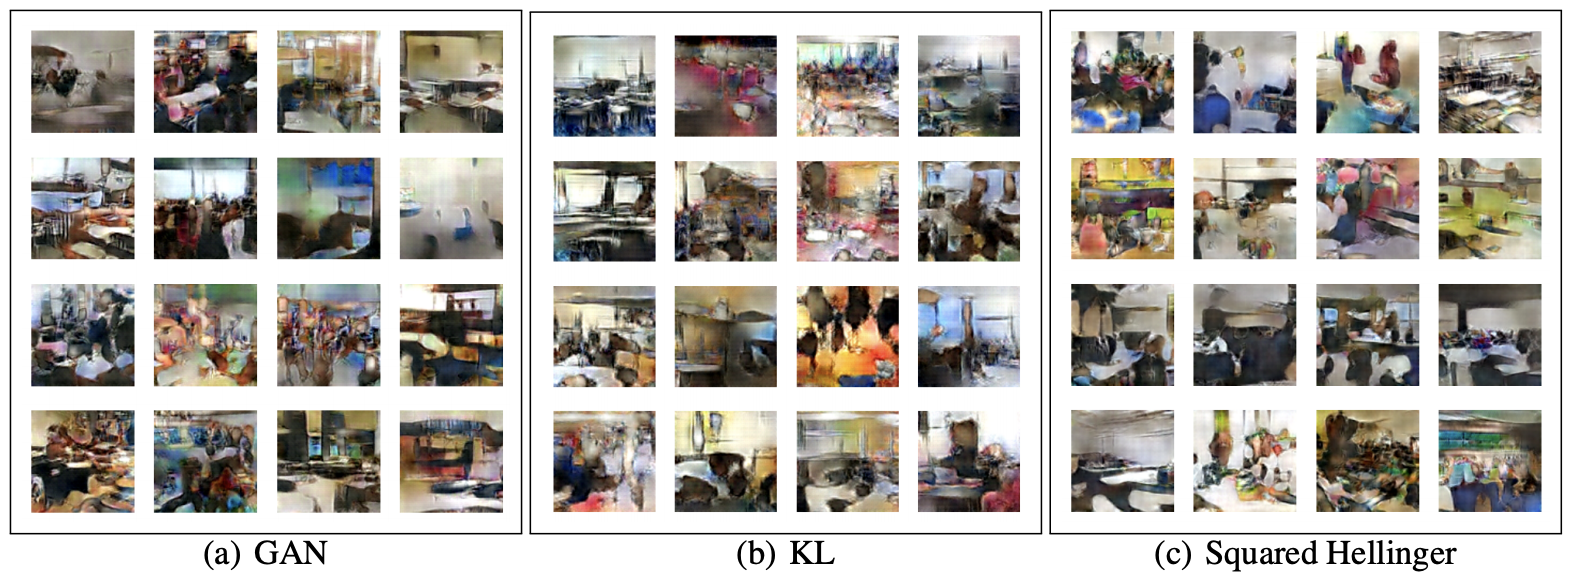
\includegraphics[width=1.0\linewidth]{figs/f_div_results}
	\end{figure}
	\vfill
	\hrule\medskip 
	{\scriptsize \href{https://arxiv.org/abs/1606.00709}{https://arxiv.org/abs/1606.00709}}
\end{frame}
%=======
\begin{frame}{Evaluation of likelihood-free models}
	How to evaluate generative models?
	\begin{block}{Likelihood-based models}
		\begin{itemize}
			\item Split data to train/val/test.
			\item Fit model on the train part.
			\item Tune hyperparameters on the validation part.
			\item Evaluate generalization by reporting likelihoods on the test set.
		\end{itemize}
	\end{block}
	\begin{block}{Not all models have tractable likelihoods}
		\begin{itemize}
			\item VAE: compare ELBO values.
			\item GAN: ???
		\end{itemize}
	\end{block}
\end{frame}
%=======
\begin{frame}{Evaluation of likelihood-free models}
	Let take some pretrained image classification model to get the conditional label distribution $p(y | \bx)$ (e.g. ImageNet classifier).
	\begin{block}{What do we want from samples?}
		\begin{itemize}
			\item \textbf{Sharpness}
			\begin{figure}
				\centering
				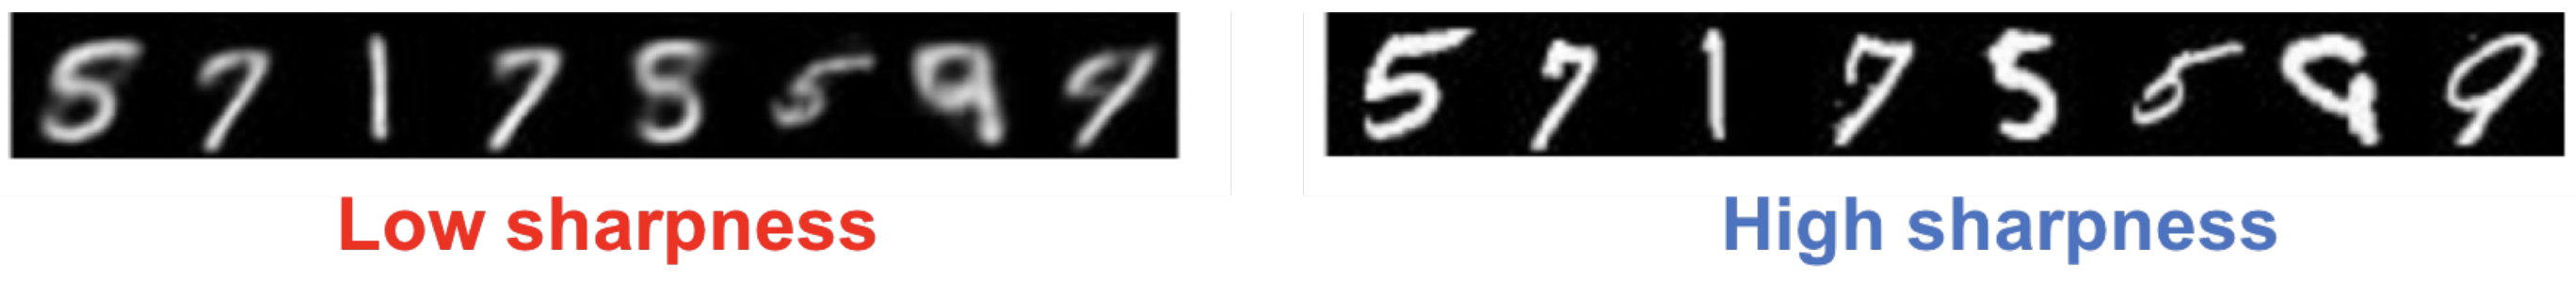
\includegraphics[width=0.9\linewidth]{figs/sharpness}
			\end{figure}
			The conditional distribution $p(y | \bx)$ should have low entropy (each image $\bx$ should have distinctly recognizable object).
			\item \textbf{Diversity}
			\begin{figure}
				\centering
				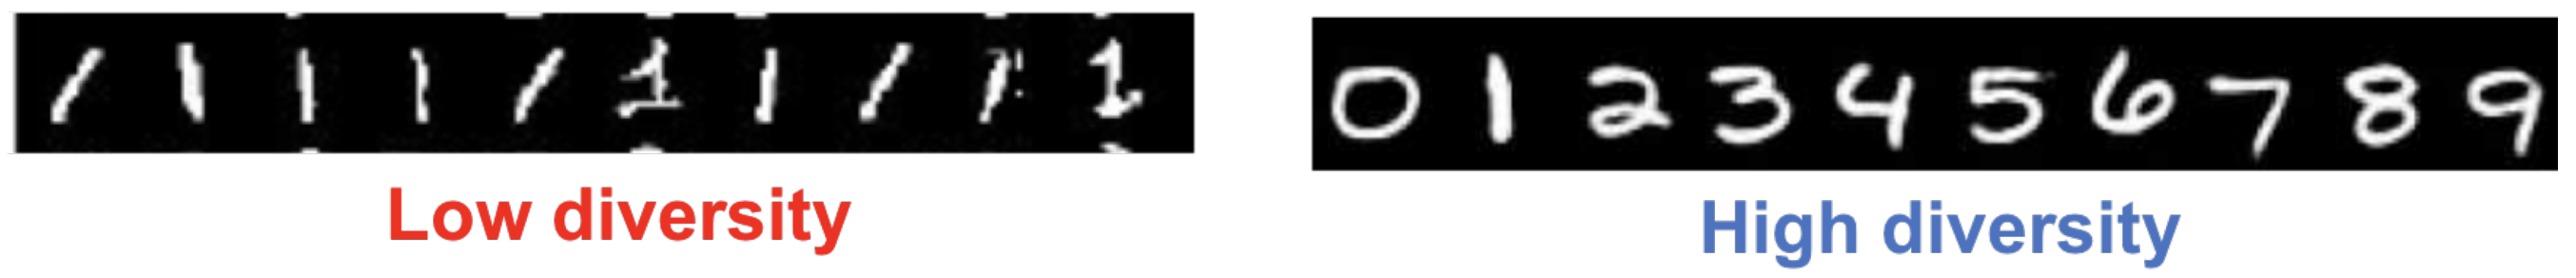
\includegraphics[width=0.9\linewidth]{figs/diversity}
			\end{figure}
			The marginal distribution $p(y) = \int p(y | \bx) p(\bx) d \bx$ should have high entropy (there should be as many classes generated as possible).
		\end{itemize}
	\end{block}
	\vfill
	\hrule\medskip 
	{\scriptsize \href{https://deepgenerativemodels.github.io}{https://deepgenerativemodels.github.io}}
\end{frame}
%=======
\begin{frame}{Evaluation of likelihood-free models}
	\begin{block}{What do we want from samples?}
		\begin{itemize}
			\item \textbf{Sharpness.}
			The conditional distribution $p(y | \bx)$ should have low entropy (each image $\bx$ should have distinctly recognizable object).
			\item \textbf{Diversity.}
			The marginal distribution $p(y) = \int p(y | \bx) p(\bx) d \bx$ should have high entropy (there should be as many classes generated as possible).
		\end{itemize}
	\end{block}
	\begin{figure}
		\centering
		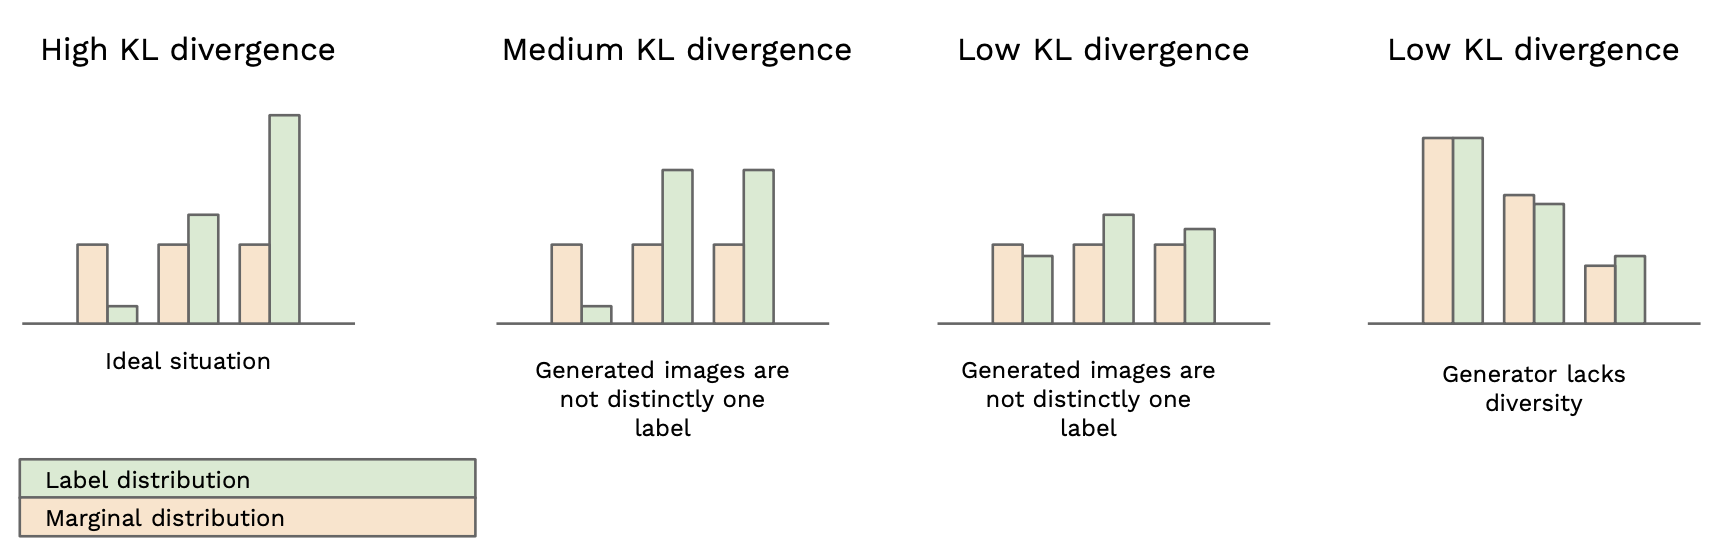
\includegraphics[width=1.0\linewidth]{figs/is_toy}
	\end{figure}
	\vfill
	\hrule\medskip 
	{\scriptsize \href{https://medium.com/octavian-ai/a-simple-explanation-of-the-inception-score-372dff6a8c7a}{https://medium.com/octavian-ai/a-simple-explanation-of-the-inception-score-372dff6a8c7a}}
\end{frame}
%=======
\begin{frame}{Evaluation of likelihood-free models}
		\begin{block}{What do we want from samples?}
		\begin{itemize}
			\item Sharpness $\Rightarrow$ low $H(y | \bx) = - \sum_{y} \int_{\bx} p(y, \bx) \log p(y | \bx) d\bx$.
			\item Diversity $\Rightarrow$ high $H(y)  = - \sum_{y} p(y) \log p(y)$.
		\end{itemize}
	\end{block}
	\begin{block}{Inception Score}
		\vspace{-0.3cm}
		\footnotesize
		\begin{align*}
			IS &= \exp(H(y) - H(y | \bx)) \\ 
			&= \exp \left( - \sum_{y} p(y) \log p(y) + \sum_{y} \int_{\bx} p(y, \bx) \log p(y | \bx) d\bx\right) \\
			&= \exp \left( \sum_{y} \int_{\bx} p(y, \bx) \log \frac{p(y | \bx)}{p(y)} d\bx\right) \\ 
			&= \exp \left( \bbE_{\bx} \sum_{y} p(y | \bx) \log \frac{p(y | \bx)}{p(y)} \right) = \exp \left( \bbE_{\bx} KL(p(y | \bx) || p(y)) \right)
		\end{align*}
	\end{block}
	\vfill
	\hrule\medskip 
	{\scriptsize \href{https://arxiv.org/abs/1606.03498}{https://arxiv.org/abs/1606.03498}}
\end{frame}
%=======
\begin{frame}{Evaluation of likelihood-free models}
	\begin{block}{Inception Score}
		\vspace{-0.1cm}
		\[
			IS =  \exp \left( \bbE_{\bx} KL(p(y | \bx) || p(y)) \right)
		\]
		\vspace{-0.1cm}
	\end{block}
	\begin{block}{IS limitations}
		\begin{itemize}
			\item Inception score depends on the quality of the pretrained classifier $p(y | \bx)$.
			\item If generator produces images with a different set of labels from the classifier training set, IS will be low.
			\item If the generator produces one image per class, the IS will be perfect (there is no measure of intra-class diversity).
			\item IS only require samples from the generator and do not take into account the desired data distribution $\pi(\bx)$ directly (only implicitly via a classifier).
		\end{itemize}
	\end{block}
	\vfill
	\hrule\medskip 
	{\scriptsize \href{https://arxiv.org/abs/1801.01973}{https://arxiv.org/abs/1801.01973}}
\end{frame}
%=======
\begin{frame}{Evaluation of likelihood-free models}
	\begin{block}{Theorem}
		If $\pi(\bx)$ and $p(\bx | \btheta)$ has moment generation functions then
		\[
			\pi(\bx) = p(\bx | \btheta) \, \Leftrightarrow \, \bbE_{\pi} \bx^k = \bbE_{p} \bx^k, \quad \forall k \geq 1.
		\]
	\end{block}
	This is intractable to calculate all moments.
	\begin{block}{Frechet Inception Distance}
		\vspace{-0.1cm}
		\[
			D^2 (\pi, p) = \| \mathbf{m}_{\pi} - \mathbf{m}_{p}\|_2^2 + \text{Tr} \left( \bC_{\pi} + \bC_p - 2 \sqrt{\bC_{\pi} \bC_p} \right)
		\]
	\end{block}
	\begin{itemize}
		\item $\mathbf{m}_{\pi}$, $\bC_{\pi} $ are mean vector and covariance matrix of feature representations for real samples from $\pi(\bx)$
		\item $\mathbf{m}_{p}$, $\bC_p$ are mean vector and covariance matrix of feature representations for generated samples from $p(\bx | \btheta)$.
		\item Representations are output of intermediate layer from pretrained classification model.
	\end{itemize} 

	\vfill
	\hrule\medskip 
	{\scriptsize \href{https://arxiv.org/abs/1706.08500}{https://arxiv.org/abs/1706.08500}}
\end{frame}
%=======
\begin{frame}{Evaluation of likelihood-free models}
	\begin{figure}
		\centering
		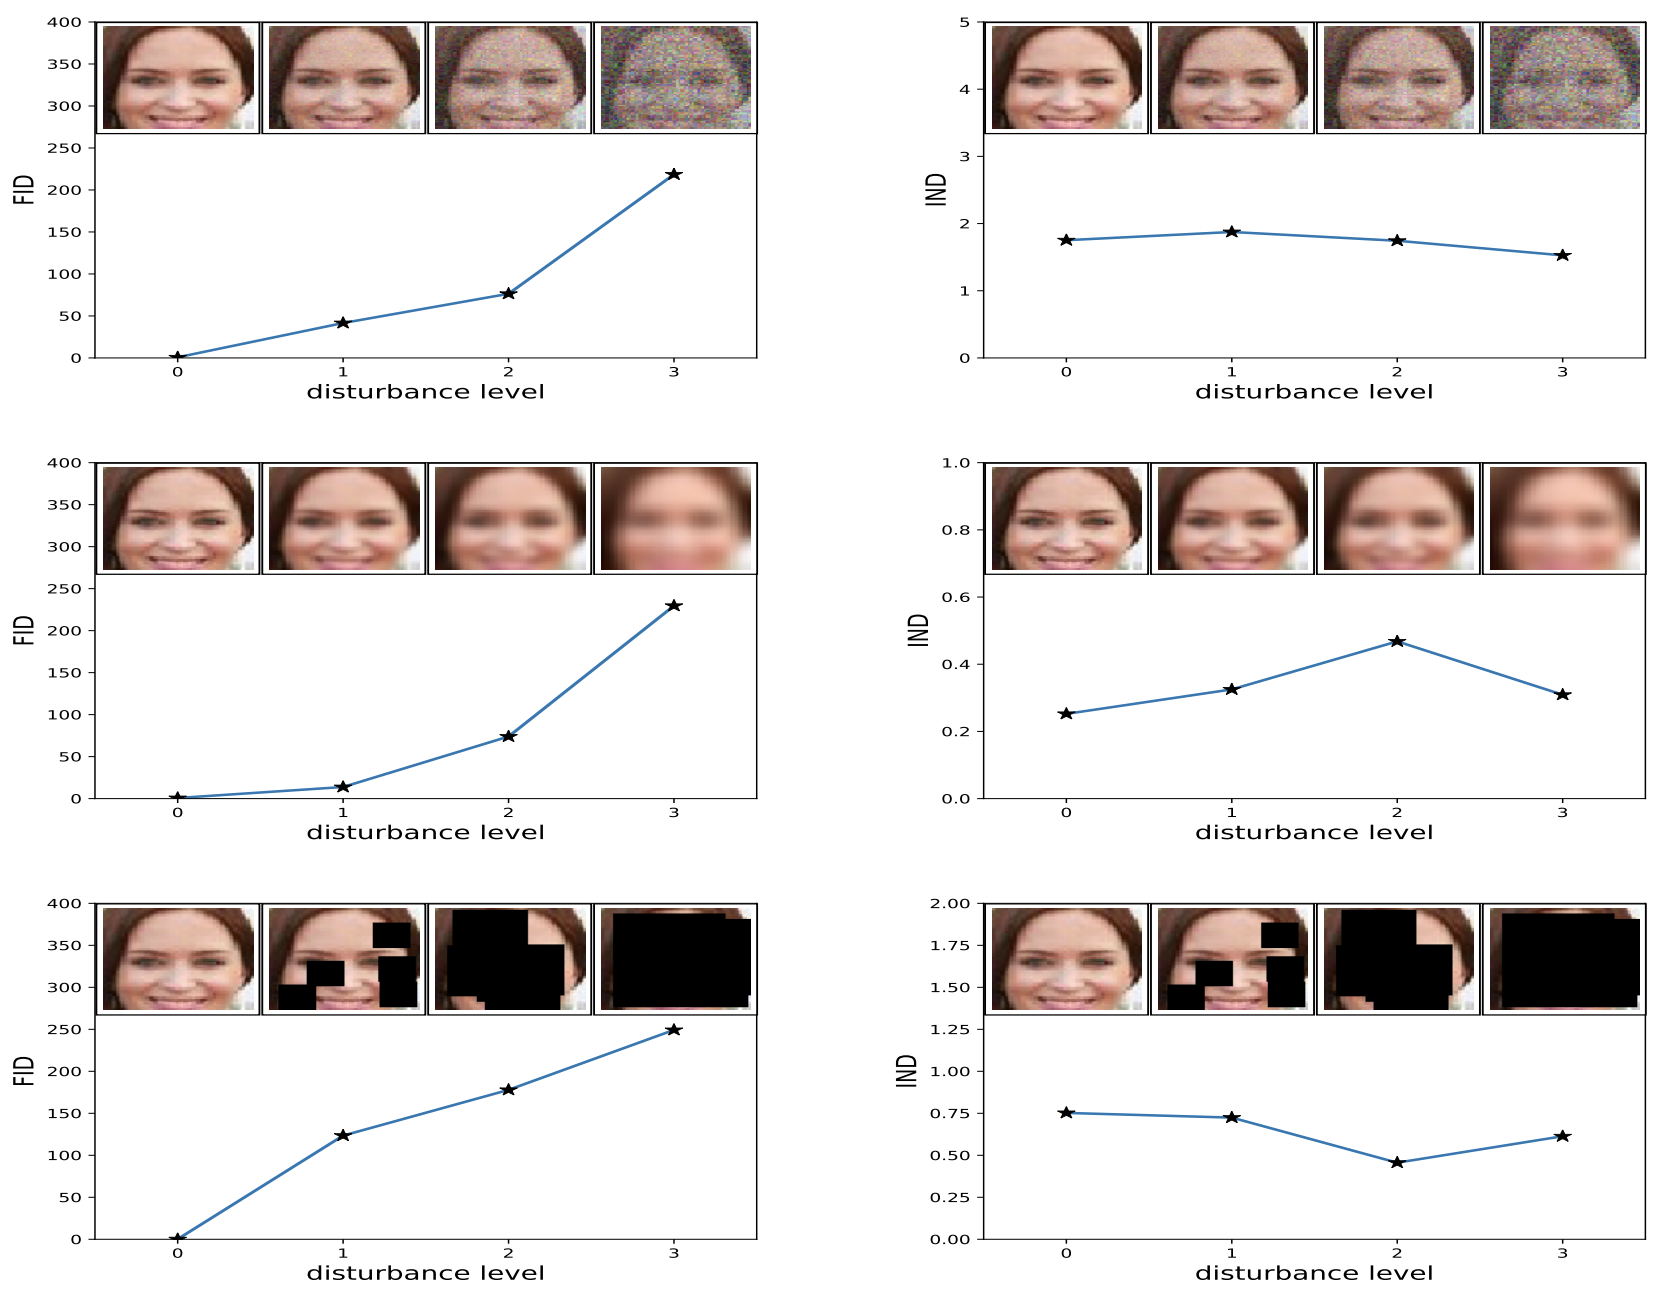
\includegraphics[width=0.9\linewidth]{figs/fid_results}
	\end{figure}
	\vfill
	\hrule\medskip 
	{\scriptsize \href{https://arxiv.org/abs/1706.08500}{https://arxiv.org/abs/1706.08500}}
\end{frame}
%=======
\begin{frame}{Evaluation of likelihood-free models}
	\begin{block}{Frechet Inception Distance}
		\vspace{-0.1cm}
		\[
		D^2 (\pi, p) = \| \mathbf{m}_{\pi} - \mathbf{m}_{p}\|_2^2 + \text{Tr} \left( \bC_{\pi} + \bC_p - 2 \sqrt{\bC_{\pi} \bC_p} \right)
		\]
	\end{block}
	\begin{block}{FID limitations}
		\begin{itemize}
			\item FID depends on the pretrained classification model.
			\item FID needs a large samples  size for evaluation.
			\item Calculation of FID is slow.
			\item FID extimates only two sample moments.
		\end{itemize}
	\end{block}
	\vspace{2cm}

	\vfill
	\hrule\medskip 
	{\scriptsize \href{https://arxiv.org/abs/1706.08500}{https://arxiv.org/abs/1706.08500}}
\end{frame}
%=======
\begin{frame}{Summary}
	\begin{itemize}
		\item Wasserstein GAN uses Kantorovich-Rubinstein duality to estimate Wasserstein distance.
		\item Gradient Penalty proposes the regularizer to enforce Lipschitzness.
		\item Spectral normalization is a weight normalization technique to enforce Lipshitzness.
		\item f-divergence family is a unified framework for divergence minimization.
		\item Inception Score and Frechet Inception Distance are the common metrics for GAN evaluation.
	\end{itemize}
\end{frame}
%=======
\begin{frame}{References}
{\tiny
\begin{itemize}
	
	\item \textbf{WGAN}: Wasserstein GAN \\
	\href{https://arxiv.org/abs/1701.07875}{https://arxiv.org/abs/1701.07875} \\
	\textbf{Summary:} Proposed Earth-Mover distance as divergence measure. It shows theoretically that EM distance could be better \\ than KL, JS and TV measures. Kantorovich-Rubinstein duality gives the new objective. All we need to enforce is Lipschitz \\ continuity (e.x. by gradient clipping).
	
	\item \textbf{WGAN-GP}: Improved Training of Wasserstein GANs \\
	\href{https://arxiv.org/abs/1704.00028}{https://arxiv.org/abs/1704.00028} \\
	\textbf{Summary:} Proves that optimal critic has unit gradient almost everywhere. Gradient penalty proposed to enforce Lipchitzness and constraint the critic norm. It greatly improves stability.
	
	\item \textbf{SN-GAN}: Spectral Normalization for Generative Adversarial Networks \\
	\href{https://arxiv.org/abs/1802.05957}{https://arxiv.org/abs/1802.05957} \\
	\textbf{Summary:} Constrain Lipschitz norm by spectral norm pf weights. Spectral norm of superpositionis less or equal to spectral norms product. Usually works better than WGAN-GP. 
	
	\item \textbf{f-GAN}:  Training generative neural samplers using variational divergence minimization  \\
	\href{https://arxiv.org/abs/1606.00709}{https://arxiv.org/abs/1606.00709} \\
	\textbf{Summary:} Extend adversarial learning pipeline to any f-divergence. Variational divergence minimization frameworkis derived. 
	
	\item Improved Techniques for Training GANs \\
	\href{https://arxiv.org/abs/1606.03498}{https://arxiv.org/abs/1606.03498} \\
	\textbf{Summary:} Inception Score for GAN evaluation was proposed.
	
	\item A Note on the Inception Score \\
	\href{https://arxiv.org/abs/1801.01973}{https://arxiv.org/abs/1801.01973} \\
	\textbf{Summary:} Inception Score is not an ideal metric.
	
	\item GANs Trained by a Two Time-Scale Update Rule Converge to a Local Nash Equilibrium \\
	\href{https://arxiv.org/abs/1706.08500}{https://arxiv.org/abs/1706.08500} \\
	\textbf{Summary:} Frechet inception distance was proposed for GAN evaluation.
\end{itemize}
}
\end{frame}
%=======
\end{document} 